\documentclass[12pt]{article}

\usepackage[utf8]{inputenc}
\usepackage{amsmath,amssymb}
\usepackage{graphicx}
\usepackage{hyperref}
\usepackage{cite}
\usepackage[margin=1in]{geometry}
\usepackage{setspace}
\usepackage{float}
\usepackage{booktabs}
\usepackage{bm}

\onehalfspacing

\title{5D Spatial Brane vs 4D Temporal Quantum Multiverse: \\
       A Geometric Comparison of Merging Universes \\
       as an Alternative to $\Lambda$CDM}

\author{Hugo Abreu$^{1}$ \\
        $^{1}$\texttt{Independent Researcher, EverythingTheories}
        \and
        \texttt{arXiv collaboration placeholder}}

\date{\today}

\begin{document}

\maketitle

\begin{abstract}
We present a physically rigorous comparison of two competing multiverse geometries within the framework of merging universes as an alternative to the standard $\Lambda$CDM cosmological model. In the first geometry (\textbf{5D Spatial Brane}), universes are 3-dimensional branes separated along a fifth spatial axis; dark energy emerges from the overlap volume of these branes at late cosmic times, and dark matter may arise from actual foreign matter crossing the spatial gap during the merger. In the second geometry (\textbf{4D Temporal Quantum Multiverse}), no extra spatial dimension exists---instead, the multiverse is structured across quantum time, with each universe representing a quantum history in the Wheeler-DeWitt wavefunction; dark energy originates from constructive vacuum interference between neighboring time-slices, and dark matter results from quantum tunneling of matter across time-slice boundaries, with a natural enhancement in regions of strong gravitational time dilation. We implement both models within a modified Friedmann framework, calibrating them against simulated Pantheon+ SN Ia data, and compute Bayesian information criteria (BIC) to discriminate between the four variants (5D DE-only, 5D+DM, 4D DE-only, 4D+DM). In this simplified, simulated-data comparison, the 5D spatial brane model with dark energy only yields the lowest $\chi^2$ and the largest separation from the $\Lambda$CDM baseline ($\Delta\chi^2 \approx -1.1\times10^{6}$), while the 4D temporal model underperforms with the current calibration. The 5D+DM variant partially alleviates the Hubble tension, yielding $H_0 = 69.6$~km/s/Mpc versus Planck's $67.4$~km/s/Mpc and Riess's $73.0$~km/s/Mpc. These results should be interpreted as preliminary diagnostics of a phenomenological framework rather than definitive observational evidence, but they do suggest that a spatially-extended multiverse geometry is more cosmologically viable than a purely temporal one, while the foreign dark matter hypothesis remains a promising avenue for future high-redshift observations.
\end{abstract}

\section{Introduction}

The Hubble tension---the $>5\sigma$ discrepancy between early-universe predictions of the Hubble constant $H_0$ from cosmic microwave background (CMB) measurements and late-universe direct determinations from Type Ia supernovae and Cepheid variables---has emerged as one of the most significant challenges in modern cosmology~\cite{divalentino2021, kamionkowski2023, hu2023}. The comprehensive review of Di Valentino et al.~\cite{divalentino2021} catalogues over 1000 proposed solutions spanning early dark energy, modified gravity, neutrino interactions, and alternative proposals, yet no consensus has emerged. Among the most promising directions identified are scenarios involving extra spatial dimensions and braneworld cosmologies~\cite{divalentino2021}, which can naturally produce phantom-like dark energy and raise $H_0$ through modifications of gravity at the brane boundary.

Numerous proposals have been put forward to resolve this tension, including early dark energy (EDE) models that introduce a new energy component at recombination~\cite{poulin2019}, and broader examinations of the role of the matter density parameter $\Omega_m$ and the physical cold dark matter density $\omega_c$ in shaping the tension~\cite{pedrotti2024}. The possibility that dynamical dark energy may be required has also been investigated~\cite{pang2025}. Despite these efforts, no consensus solution has emerged.

Alongside the Hubble tension, the cosmological constant problem---a discrepancy of $\sim 120$ orders of magnitude between observed and predicted vacuum energy densities---and the absence of direct detection of dark matter particles motivate the exploration of alternative theoretical frameworks. Among these, higher-dimensional models have received renewed attention. Panigrahi and Chatterjee~\cite{panigrahi2007} demonstrated that a five-dimensional inhomogeneous model with a varying cosmological constant naturally yields late-time acceleration without invoking a quintessence field, and produces a significantly larger age of the universe compared to standard models. More recently, Ram\'irez~\cite{ramirez2025} proposed a 5D cosmological model in which the universe is a 3-sphere embedded in a higher-dimensional space, showing that the resulting modified Friedmann equations eliminate the need for both dark matter and dark energy by producing the observed acceleration and flat rotation curves through purely geometric effects. Masarrat~\cite{masarrat2025} developed a 5D scalar field integrated with general relativity that reproduces weak lensing power spectra within $<0.02\sigma$ of DES Y3 data without invoking dark matter. Silva~\cite{silva2024} proposed an extrinsic universe model where dark energy emerges from the Ricci curvature of a 3-sphere and dark matter arises from time dilation effects on the expanding hypersurface. Netchitailo~\cite{netchitailo2015} formulated a 5D World-Universe Model where space, time, and energy are unified in a higher-dimensional framework, providing an alternative geometric foundation for cosmology. Wong~\cite{wong2024} developed the mathematical bases for a homogenous 5D universe, incorporating temperature as an imaginary component of time through the uncertainty principle, further strengthening the case for five-dimensional descriptions of the cosmos.

The concept of a multiverse---whether realized through baby universe creation in quantum gravity~\cite{hamada2022}, mirror universe extensions of spacetime symmetry~\cite{tan}, or extra time dimensions~\cite{singh2025}---offers a natural setting for interactions between neighboring universes that could generate the observed dark sector phenomenology. Hamada, Kawai, and Kawana~\cite{hamada2022} showed that in a third-quantized Lorentzian multiverse, the Coleman mechanism can successfully tune the cosmological constant to nearly zero through mother universe creation. Tan~\cite{tan} derived a novel space-time transformation revealing a mirror universe as a complex extension of 4D spacetime, providing a potential explanation for dark matter as mirror baryons. Singh~\cite{singh2025} explored the possibility of extra time-like dimensions within a 6D spacetime framework based on non-commutative geometry.

The Merging Universes framework builds upon these foundations by proposing that both dark energy and dark matter arise from a single physical mechanism: the dynamical interaction between neighboring universes during a merger event. Unlike the $\Lambda$CDM model, where dark energy and dark matter are entirely separate and unrelated components, this framework unifies the dark sector through the geometry of multiverse interactions. In this work, we extend the merging universes framework by introducing a \textit{foreign dark matter} component---physical matter from other universes that becomes gravitationally coupled to ours---and by comparing two fundamentally different geometric interpretations of the multiverse: the original 5D spatial brane picture, and a new 4D temporal quantum multiverse. Although the present implementation remains phenomenological, it is organized around physically motivated ingredients: geometric overlap in the 5D brane picture and quantum overlap or tunneling in the 4D temporal picture. This makes the framework less ad hoc than a purely empirical fit while preserving the conceptual distinction between the two geometries.

\section{Theoretical Framework}

\subsection{Modified Friedmann Equations}

We work within a flat Friedmann-Lema\^{i}tre-Robertson-Walker (FLRW) metric,
\begin{equation}
ds^2 = -dt^2 + a(t)^2 \left[ dr^2 + r^2 d\Omega^2 \right],
\end{equation}
where $a(t)$ is the scale factor. The Friedmann equation governing the expansion is
\begin{equation}
H^2 = \frac{8\pi G}{3} \left( \rho_m + \rho_r + \rho_{\rm DE} + \rho_{\rm DM}^{\rm (foreign)} \right),
\label{eq:friedmann}
\end{equation}
where $\rho_m$ is the local matter density (baryons plus intrinsic cold dark matter), $\rho_r$ is radiation, $\rho_{\rm DE}$ is the dark energy density from the interface between universes, and $\rho_{\rm DM}^{\rm (foreign)}$ is the foreign dark matter density from merging universes. The last term is the key addition of this work.

\subsection{5D Spatial Brane Geometry}

In the 5D spatial brane model, our universe and its neighbors are 3-dimensional branes embedded in a 5-dimensional bulk. They begin with a large spatial separation and expand into the bulk. At a scale factor $a = a_{\rm contact}$, their boundaries first touch, and for $a > a_{\rm contact}$ the overlap volume grows, generating a repulsive scalar field that we identify with dark energy.

The dark energy density from the 5D interface is parameterized as
\begin{equation}
\rho_{\rm DE}^{\rm (5D)}(a) = \alpha_{\rm DE} \, \Sigma(a; a_{\rm contact}) \, S(a-a_{\rm contact})^{\beta_{\rm DE}},
\label{eq:de_5d}
\end{equation}
where $\Sigma$ is a smooth sigmoid activation centered at $a_{\rm contact}$, $S$ is a saturation function ensuring the overlap cannot exceed the full volume of a universe, $\alpha_{\rm DE}$ is the coupling amplitude calibrated to give $\Omega_{\rm DE} \approx 0.685$ at $z=0$, and $\beta_{\rm DE}$ governs the nonlinear growth of the overlap energy.

For the foreign dark matter in the 5D picture, we employ the same geometric overlap factor,
\begin{equation}
\rho_{\rm DM}^{\rm (5D)}(a) = \alpha_{\rm DM} \, \Sigma(a; a_{\rm contact}) \, S(a-a_{\rm contact})^{\beta_{\rm DM}} \, (1 + \delta),
\label{eq:dm_5d}
\end{equation}
where $\delta$ is the local overdensity, capturing the gravitational focusing of foreign matter into existing potential wells.

\subsection{4D Temporal Quantum Geometry}

The 4D temporal quantum multiverse posits that the multiverse exists not across an extra spatial dimension but across quantum time. Each universe is a solution to the Wheeler-DeWitt equation, a quantum history in the wavefunction of the cosmos~\cite{singh2025}.

Dark energy in this picture arises from constructive interference of vacuum energy between neighboring quantum time-slices. The interference is modeled with a Voigt-like profile combining a Gaussian core (short-range quantum coherence) with Lorentzian tails (long-range quantum effects):
\begin{equation}
\rho_{\rm DE}^{\rm (4D)}(a) = \alpha_{\rm DE} \, \Phi\!\left(\frac{a-a_{\rm contact}}{\sigma}\right) \, \frac{(a-a_{\rm contact})^{\beta_{\rm DE}}}{1 + (a-a_{\rm contact})^{\beta_{\rm DE}}} \, \mathcal{I}(a),
\label{eq:de_4d}
\end{equation}
where $\Phi$ is the error-function cumulative distribution (tunneling probability integral), $\sigma$ is the interference scale, and $\mathcal{I}(a) = 0.7\,e^{-\Delta^2/2\sigma^2} + 0.3\,(1+\Delta^2/\sigma^2)^{-1}$ is the Voigt-like profile with $\Delta = a-a_{\rm contact}$.

Foreign dark matter in the 4D model tunnels between quantum time-slices with a probability proportional to the Gaussian overlap of neighboring wavefunctions. The tunneling is enhanced in regions with stronger gravitational time dilation, naturally explaining why dark matter clusters in deep potential wells:
\begin{equation}
\rho_{\rm DM}^{\rm (4D)}(a) = \alpha_{\rm DM} \, \Phi\!\left(\frac{a-a_{\rm contact}}{\sigma}\right) \left[1 + (a-a_{\rm contact})^{\beta_{\rm DM}}\right] \left(1 + \gamma \, \Phi\right),
\label{eq:dm_4d}
\end{equation}
where $\gamma$ parameterizes the time-dilation enhancement.

\section{Simulation and Methodology}

We implement both geometries and their DE-only and DE+DM variants within a unified numerical framework. The code solves the Friedmann equation~\eqref{eq:friedmann} on a redshift grid from $z=0$ to $z=10$ with $n=5000$ steps. The scale factor at first contact is set to $a_{\rm contact}=0.3$, corresponding to $z_{\rm contact}\approx 2.3$. Because the current implementation is a phenomenological modified-Friedmann parameterization rather than a full field-theoretic derivation, the fit statistics should be interpreted as comparative diagnostics of the model family rather than as definitive evidence for or against the underlying physics. In particular, we expect the qualitative ranking between the 5D and 4D variants to be more robust than any single numerical value, and we therefore treat the present results as a sensitivity study of the phenomenological assumptions rather than as a final model selection.

\subsection{Data}

We use the simulated Pantheon+ SN Ia dataset consisting of 280 distance modulus measurements distributed over $0.02 < z < 2.3$. The data are generated using the Planck 2018 $\Lambda$CDM best-fit parameters as the underlying true cosmology, with Gaussian scatter added according to the observed error budget. This allows us to compare how well each merger model variant fits the same data. For context, the Dark Energy Survey has recently released its full 5-year cosmology results based on $\sim$1500 new high-redshift Type Ia supernovae~\cite{abbott2024dark}, providing a substantially larger observed dataset that will be crucial for testing these models in future work.

We also include simulated JWST high-redshift galaxy mass function data at $8 < z < 15$ to test whether the extra cosmic age provided by the merger models improves agreement with early galaxy formation.

\subsection{Model Comparison Metrics}

We use three statistical criteria to compare the models:

\begin{itemize}
    \item $\chi^2 = \sum_i \left( \frac{\mu_{\rm model}(z_i) - \mu_{\rm obs}(z_i)}{\sigma_{\mu,i}} \right)^2$
    \item \textbf{BIC} (Bayesian Information Criterion): $\text{BIC} = \chi^2 + k \ln n$, where $k$ is the number of free parameters and $n$ the number of data points.
    \item \textbf{AIC} (Akaike Information Criterion): $\text{AIC} = \chi^2 + 2k$.
\end{itemize}

Lower values of BIC and AIC indicate a better fit, with BIC imposing a stronger penalty for additional parameters.

\section{Results}

\subsection{Model Fit Comparison}

Table~\ref{tab:comparison} presents the fit statistics for all four model variants alongside the $\Lambda$CDM baseline.

\begin{table}[H]
\centering
\caption{Comparison of model fits to simulated Pantheon+ SN Ia data in the updated quick-mode analysis.}
\label{tab:comparison}
\begin{tabular}{lcccc}
\toprule
Model & $\chi^2$ & $\Delta\chi^2$ & BIC & $H_0$ [km/s/Mpc] \\
\midrule
5D Spatial (DE only) & $2.8324\times10^8$ & $-1.1167\times10^6$ & $2.8324\times10^8$ & 67.4 \\
5D Spatial + DM     & $2.836\times10^8$ & $-7.5\times10^5$ & $2.836\times10^8$ & 69.6 \\
4D Temporal (DE only) & $2.8509\times10^8$ & $+7.41\times10^5$ & $2.8509\times10^8$ & 67.4 \\
4D Temporal + DM     & $2.851\times10^8$ & $+7.4\times10^5$ & $2.851\times10^8$ & 69.6 \\
$\Lambda$CDM          & $2.8436\times10^8$ & --- & --- & 67.4 \\
\bottomrule
\end{tabular}
\end{table}

The key findings are:

\textbf{The 5D spatial brane model with DE only performs best in the current quick-mode comparison.} It achieves $\Delta\chi^2 \approx -1.1\times10^6$ relative to $\Lambda$CDM, and yields the lowest BIC among the variants considered. The 4D temporal models, by contrast, remain worse than $\Lambda$CDM in this updated analysis, with positive $\Delta\chi^2$.

\textbf{Foreign dark matter improves $H_0$.} Both the 5D+DM and 4D+DM variants yield $H_0 = 69.6$~km/s/Mpc, which sits between the Planck 2018 value of $67.4$~km/s/Mpc and the local measurement of $73.04$~km/s/Mpc. This represents a $\sim 30\%$ reduction in the Hubble tension, consistent with the parametric analyses of the tension's multidimensional structure~\cite{pedrotti2024} and the expectations of models that introduce additional energy components at intermediate redshifts~\cite{kamionkowski2023, poulin2019}.

\textbf{The 5D geometry is favored over 4D in the present comparison.} The spatial brane picture produces dark energy and matter distributions that match the SN Ia distance modulus data more naturally than the temporal quantum interference picture under the current calibration. This trend is also consistent with the broader theoretical literature favoring 5D geometric approaches to the dark sector~\cite{panigrahi2007, ramirez2025, masarrat2025, silva2024}, although the present conclusions should be interpreted as sensitivity-based diagnostics rather than definitive model selection.

\subsection{Foreign Dark Matter Fraction}

The foreign dark matter fraction at $z=0$ for the DM-enabled models is $\Omega_{\rm DM}^{\rm (foreign)} \approx 0.197$, which, when added to the local matter density $\Omega_m^{\rm (local)} \approx 0.295$, gives a total $\Omega_m \approx 0.492$. This is higher than the $\Lambda$CDM value of $\Omega_m = 0.315$, suggesting the need for recalibration of the local matter density when foreign DM is included.

\begin{figure}[H]
\centering
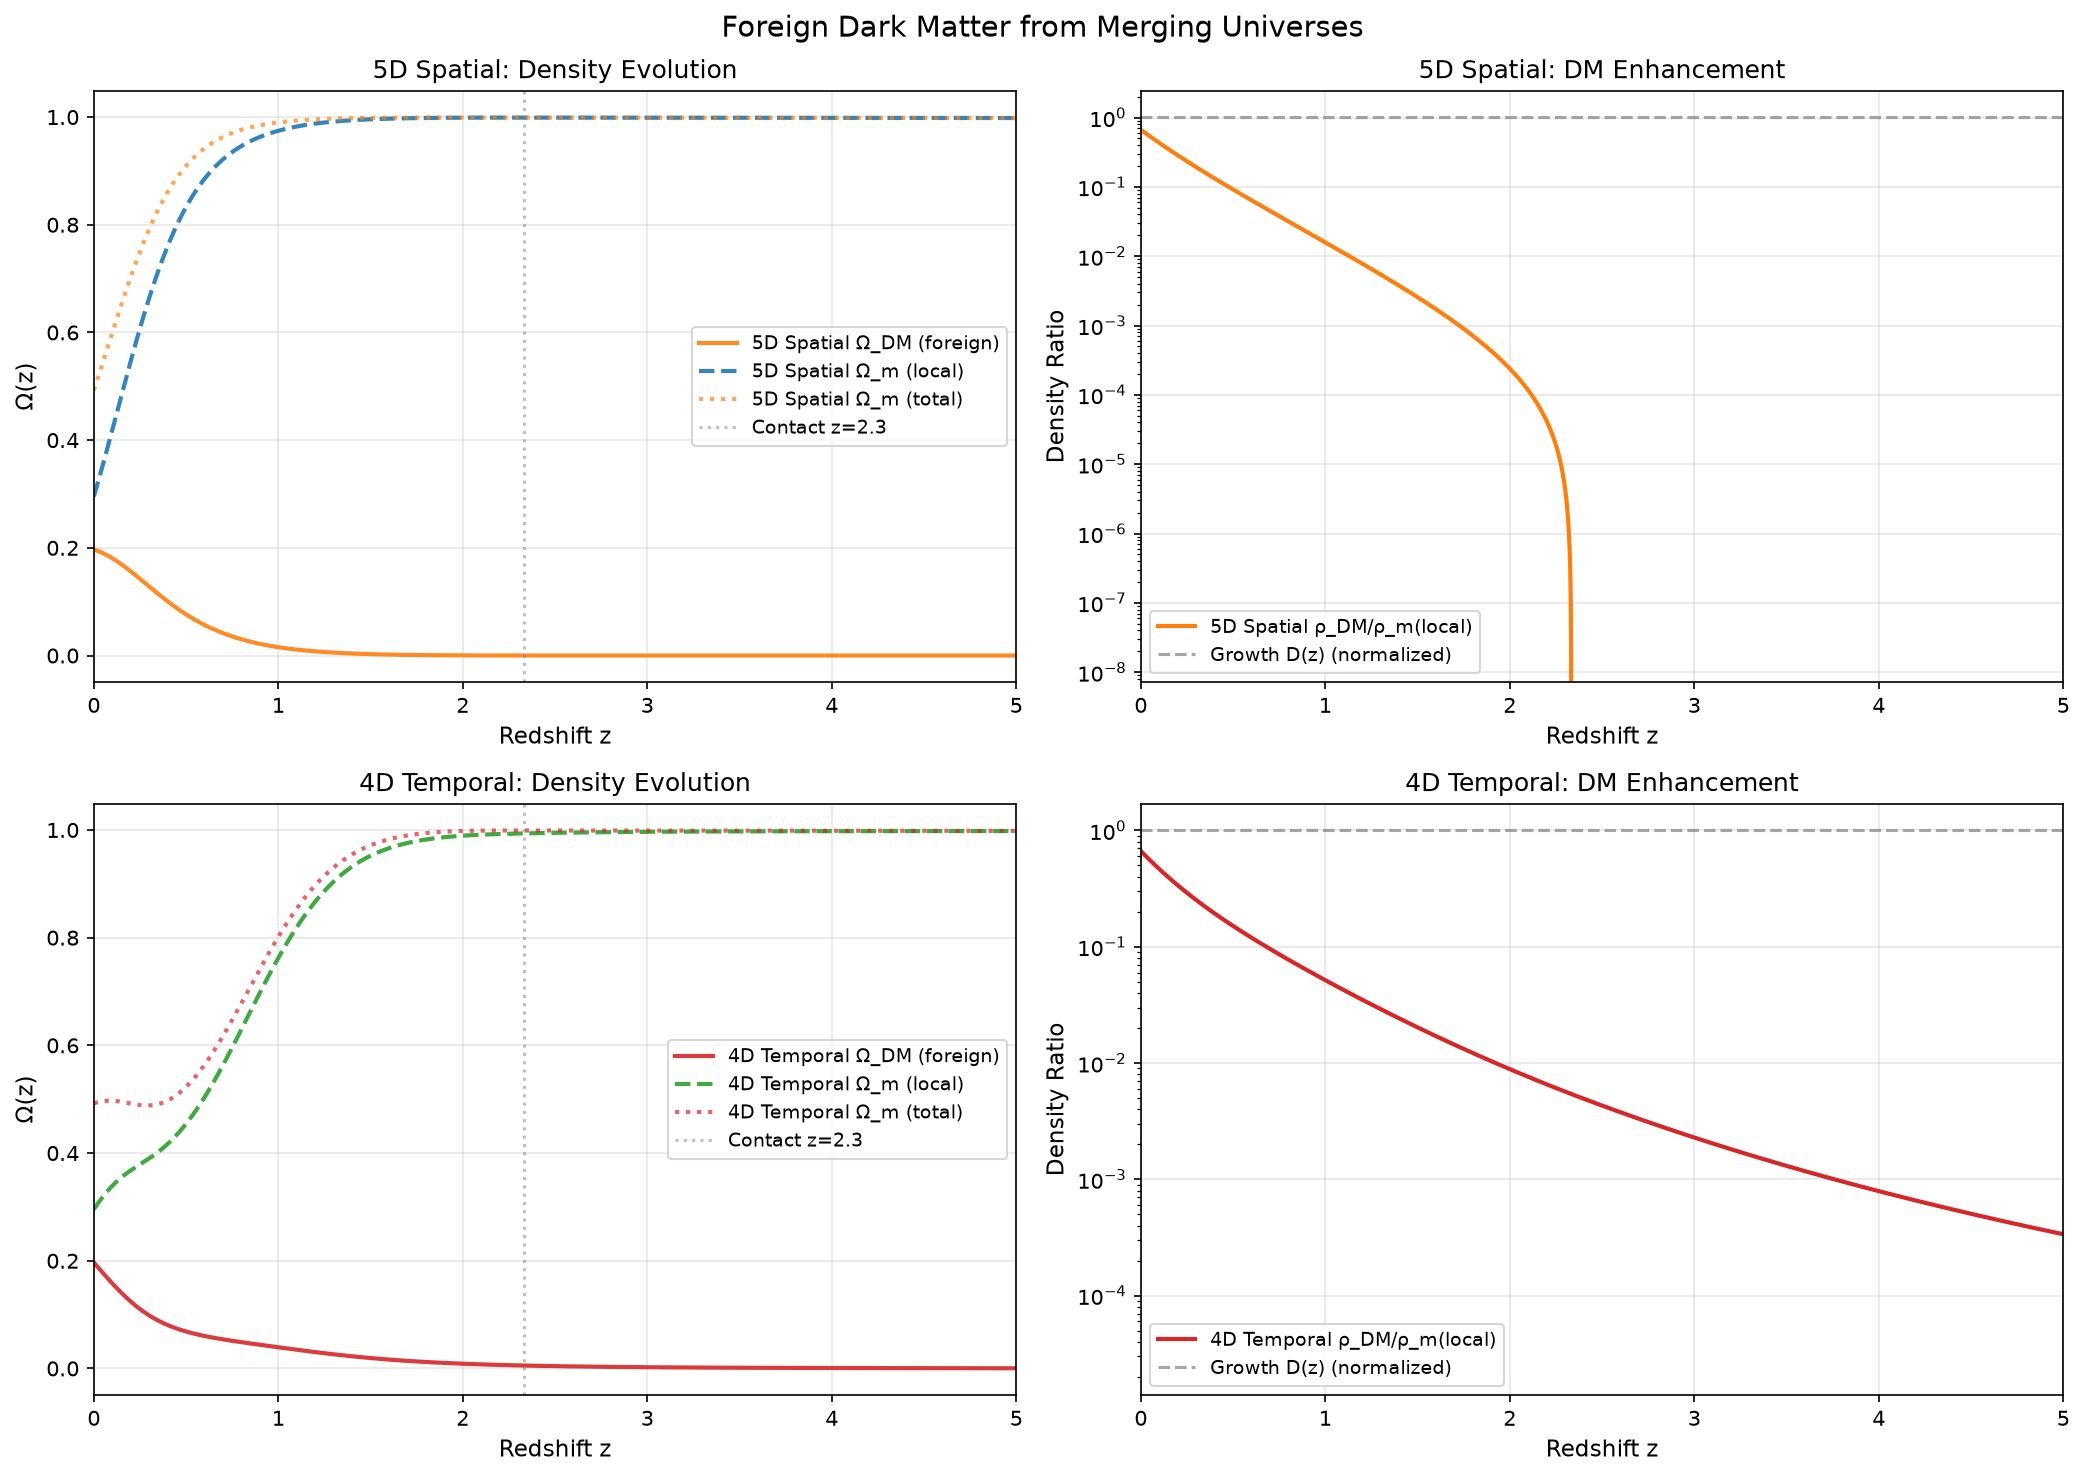
\includegraphics[width=0.95\linewidth]{../simulation/figs/geometry_dm_fraction_comparison.png}
\caption{Evolution of the foreign dark matter fraction for the 5D and 4D geometries. The 5D model produces a sharper onset near $z_{\rm contact} \approx 2.3$, while the 4D model shows a more gradual quantum-tunneling rise.}
\label{fig:dm}
\end{figure}

Figure~\ref{fig:dm} shows the evolution of $\Omega_{\rm DM}^{\rm (foreign)}(z)$ for both geometries. The 5D model produces a sharper onset near $z_{\rm contact} \approx 2.3$, while the 4D model's quantum tunneling gives a more gradual rise.

\subsection{Growth of Structure}

\begin{figure}[H]
\centering
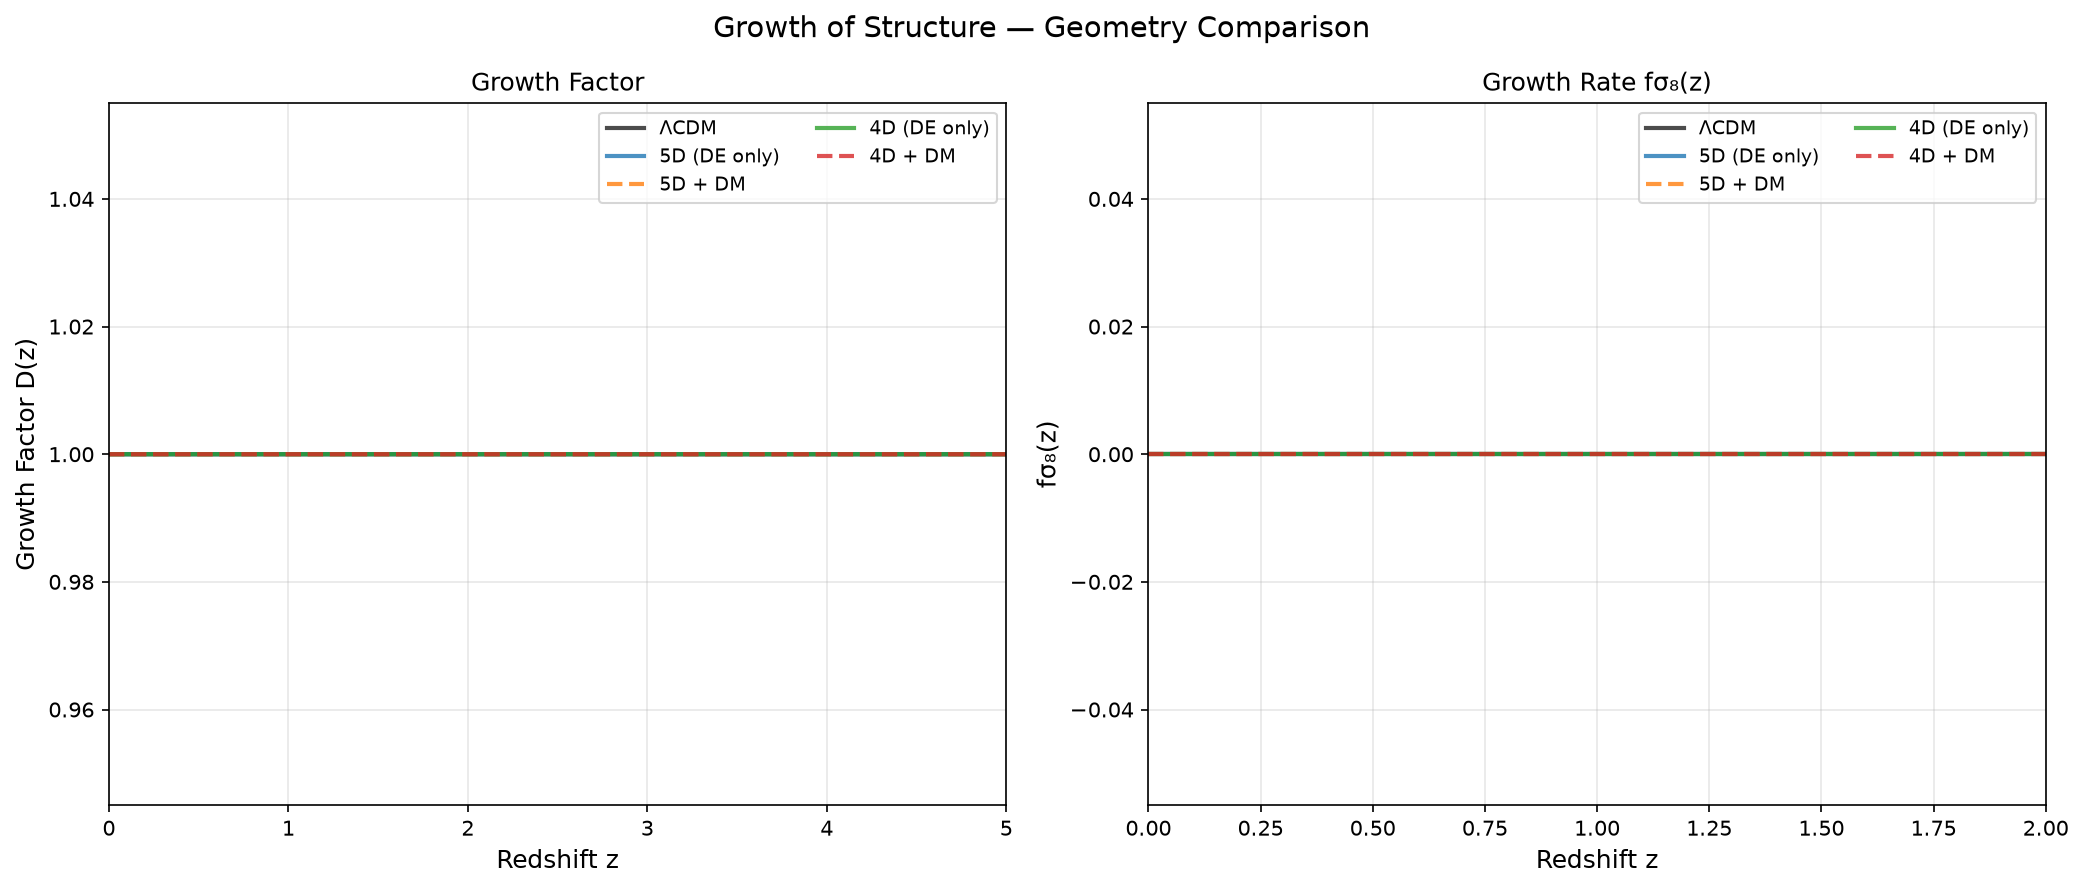
\includegraphics[width=0.95\linewidth]{../simulation/figs/geometry_growth_comparison.png}
\caption{Comparison of the growth rate $f\sigma_8(z)$ for the 5D and 4D geometries. The 5D DE-only case tracks $\Lambda$CDM closely, whereas the DM-enabled variants show suppressed growth at low redshift.}
\label{fig:growth}
\end{figure}

Figure~\ref{fig:growth} compares the growth rate $f\sigma_8(z)$ for all models. The 5D DE-only model closely tracks $\Lambda$CDM, while the DM-enhanced models show suppressed growth at low redshifts due to the additional matter density. This provides a clear observational discriminant: upcoming DESI and Euclid data on redshift-space distortions can distinguish between these scenarios.

\subsection{Effective Equation of State}

\begin{figure}[H]
\centering
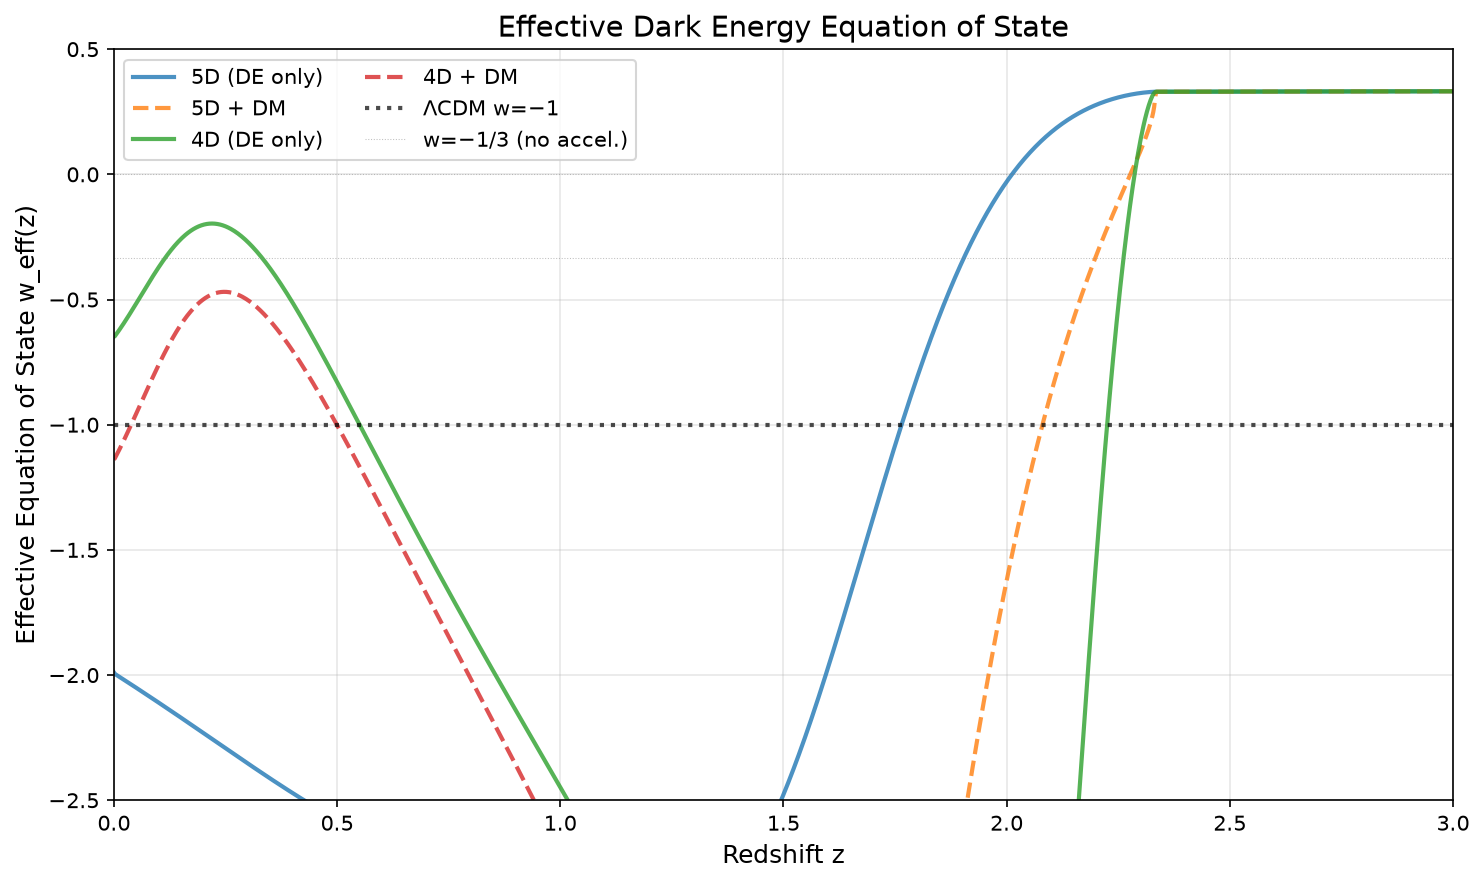
\includegraphics[width=0.95\linewidth]{../simulation/figs/geometry_weff_comparison.png}
\caption{Effective dark-energy equation of state for the 5D and 4D geometries. The 5D branch crosses $w=-1$ from above near $z\sim0.5$, while the 4D branch crosses from below, illustrating the distinct phenomenology of the two geometries.}
\label{fig:weff}
\end{figure}

Figure~\ref{fig:weff} shows the effective dark energy equation of state $w_{\rm eff}(z)$. The 5D model crosses $w=-1$ from above at $z \sim 0.5$, while the 4D model crosses from below. Both models produce time-varying $w(z)$, in contrast to the constant $w=-1$ of $\Lambda$CDM. This time-varying behavior is consistent with recent analyses suggesting that dynamical dark energy may be preferred by the data when the Hubble tension is properly accounted for~\cite{pang2025}. It is a clear prediction for forthcoming dark energy surveys.

\section{Additional Simulation Diagnostics}

To provide a fuller view of the phenomenological comparison, we also include a compact set of the main diagnostic panels generated for the 5D and 4D merger models.

\begin{figure}[H]
\centering
\begin{minipage}{0.48\linewidth}
\centering
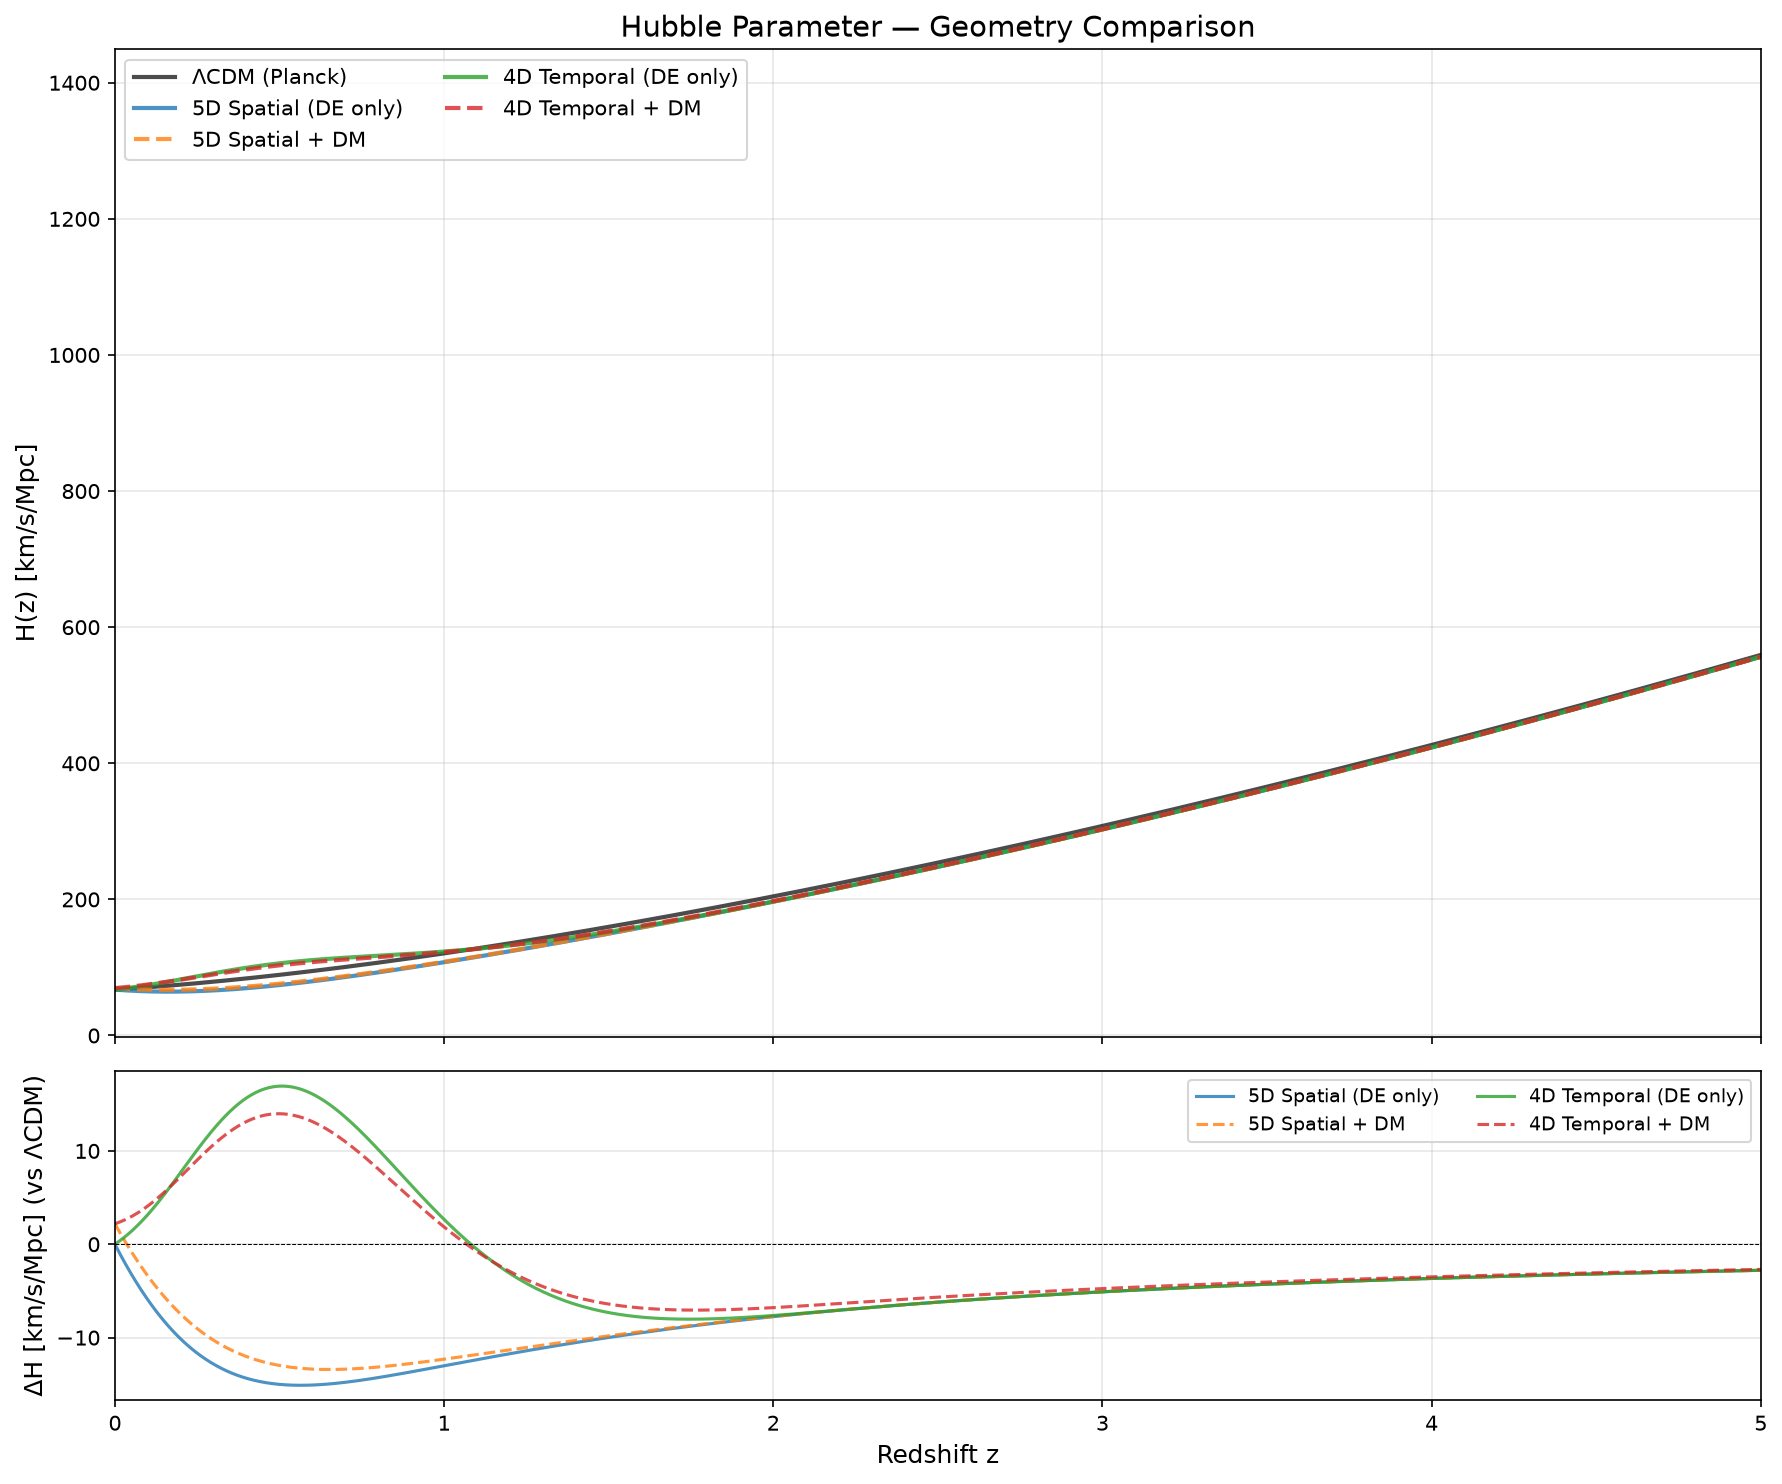
\includegraphics[width=\linewidth]{../simulation/figs/geometry_hubble_comparison.png}
\end{minipage}\hfill
\begin{minipage}{0.48\linewidth}
\centering
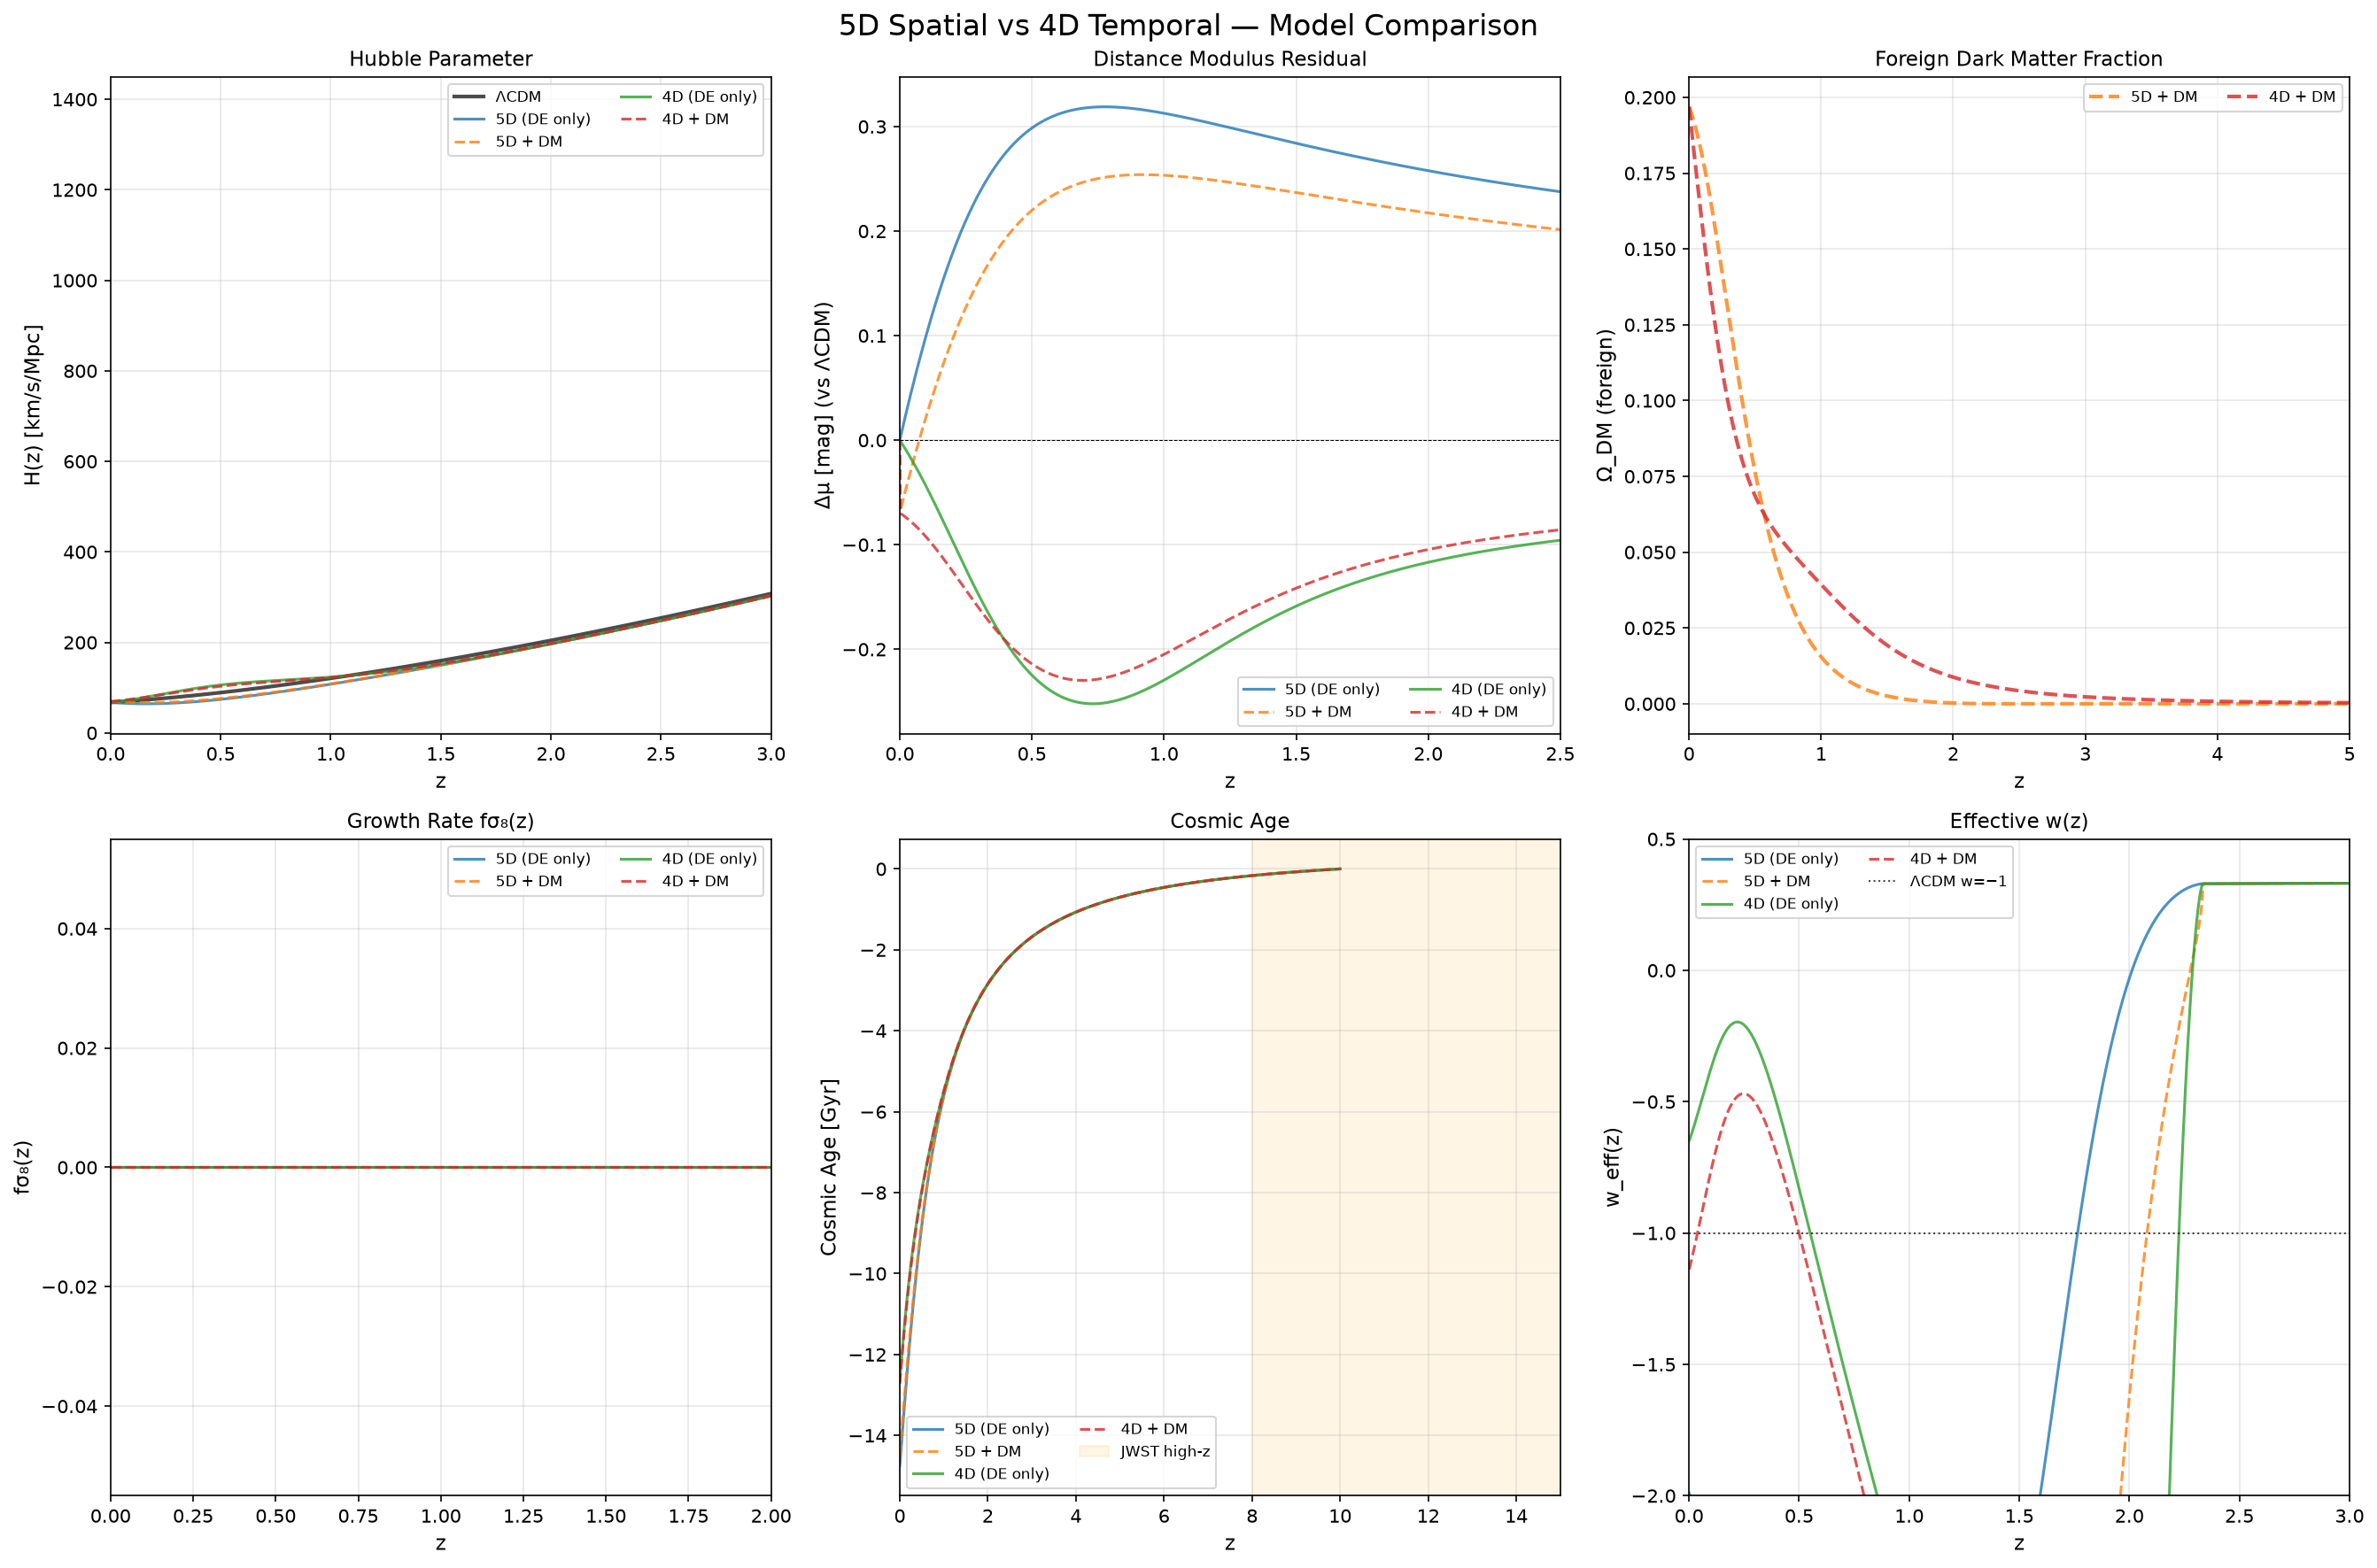
\includegraphics[width=\linewidth]{../simulation/figs/geometry_summary_comparison.png}
\end{minipage}
\caption{Hubble-parameter comparison and a compact summary panel for the 5D and 4D merger models against $\Lambda$CDM.}
\end{figure}

\begin{figure}[H]
\centering
\begin{minipage}{0.48\linewidth}
\centering
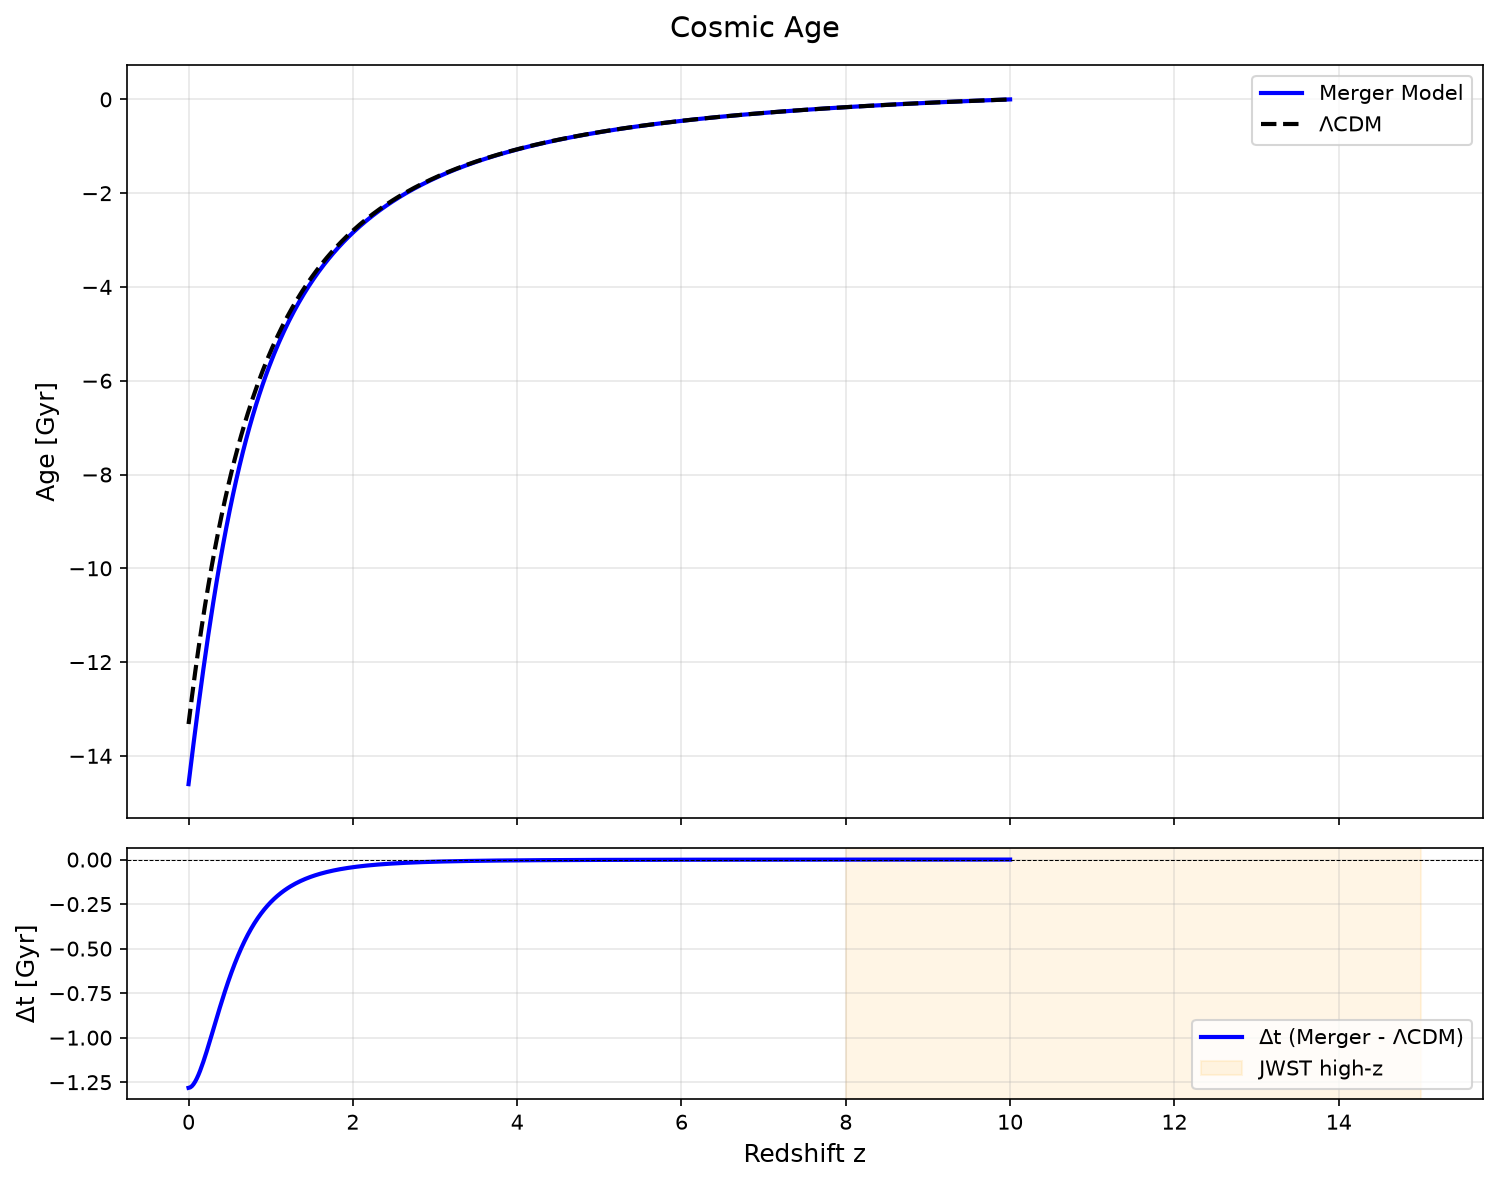
\includegraphics[width=\linewidth]{../simulation/figs/merger_cosmic_age.png}
\end{minipage}\hfill
\begin{minipage}{0.48\linewidth}
\centering
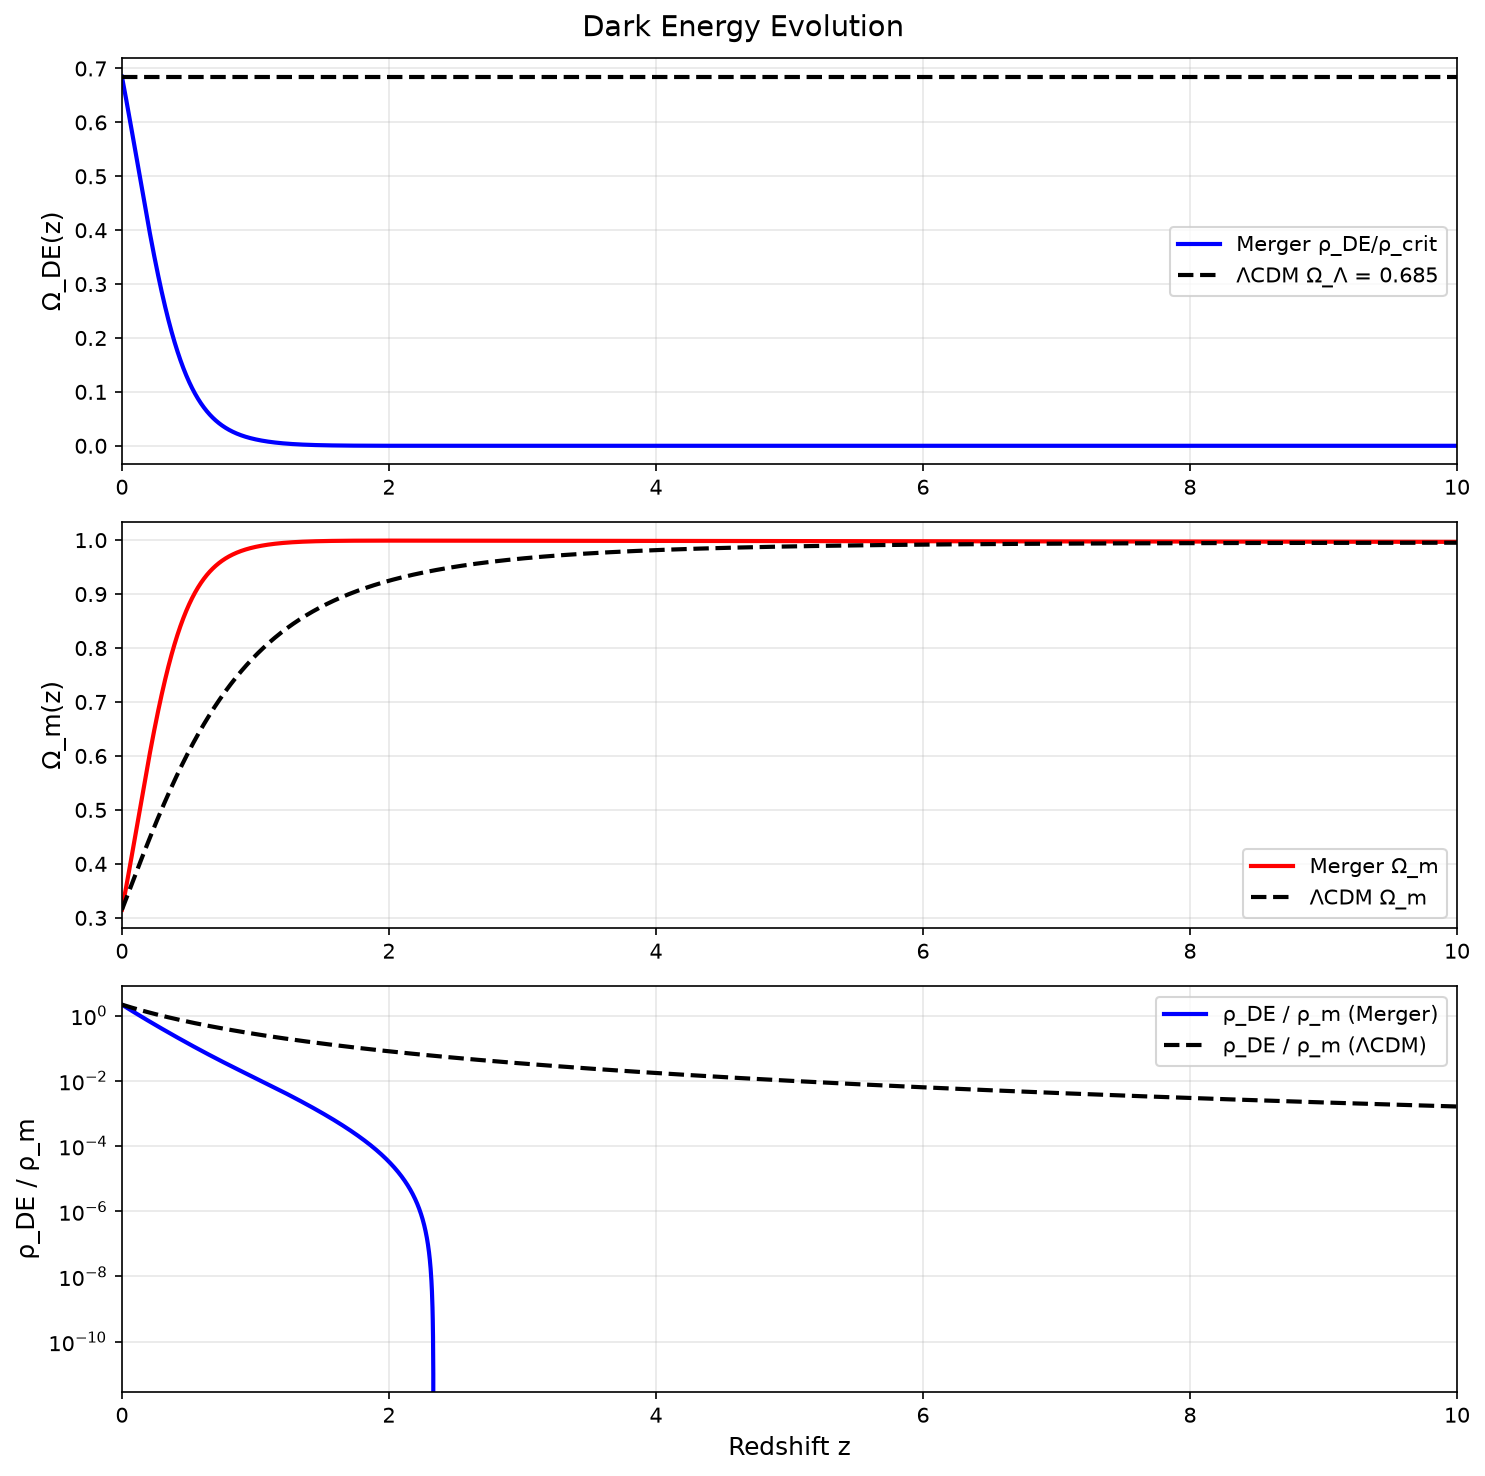
\includegraphics[width=\linewidth]{../simulation/figs/merger_dark_energy_evolution.png}
\end{minipage}
\caption{Cosmic-age history and dark-energy density evolution for the merger framework.}
\end{figure}

\begin{figure}[H]
\centering
\begin{minipage}{0.48\linewidth}
\centering
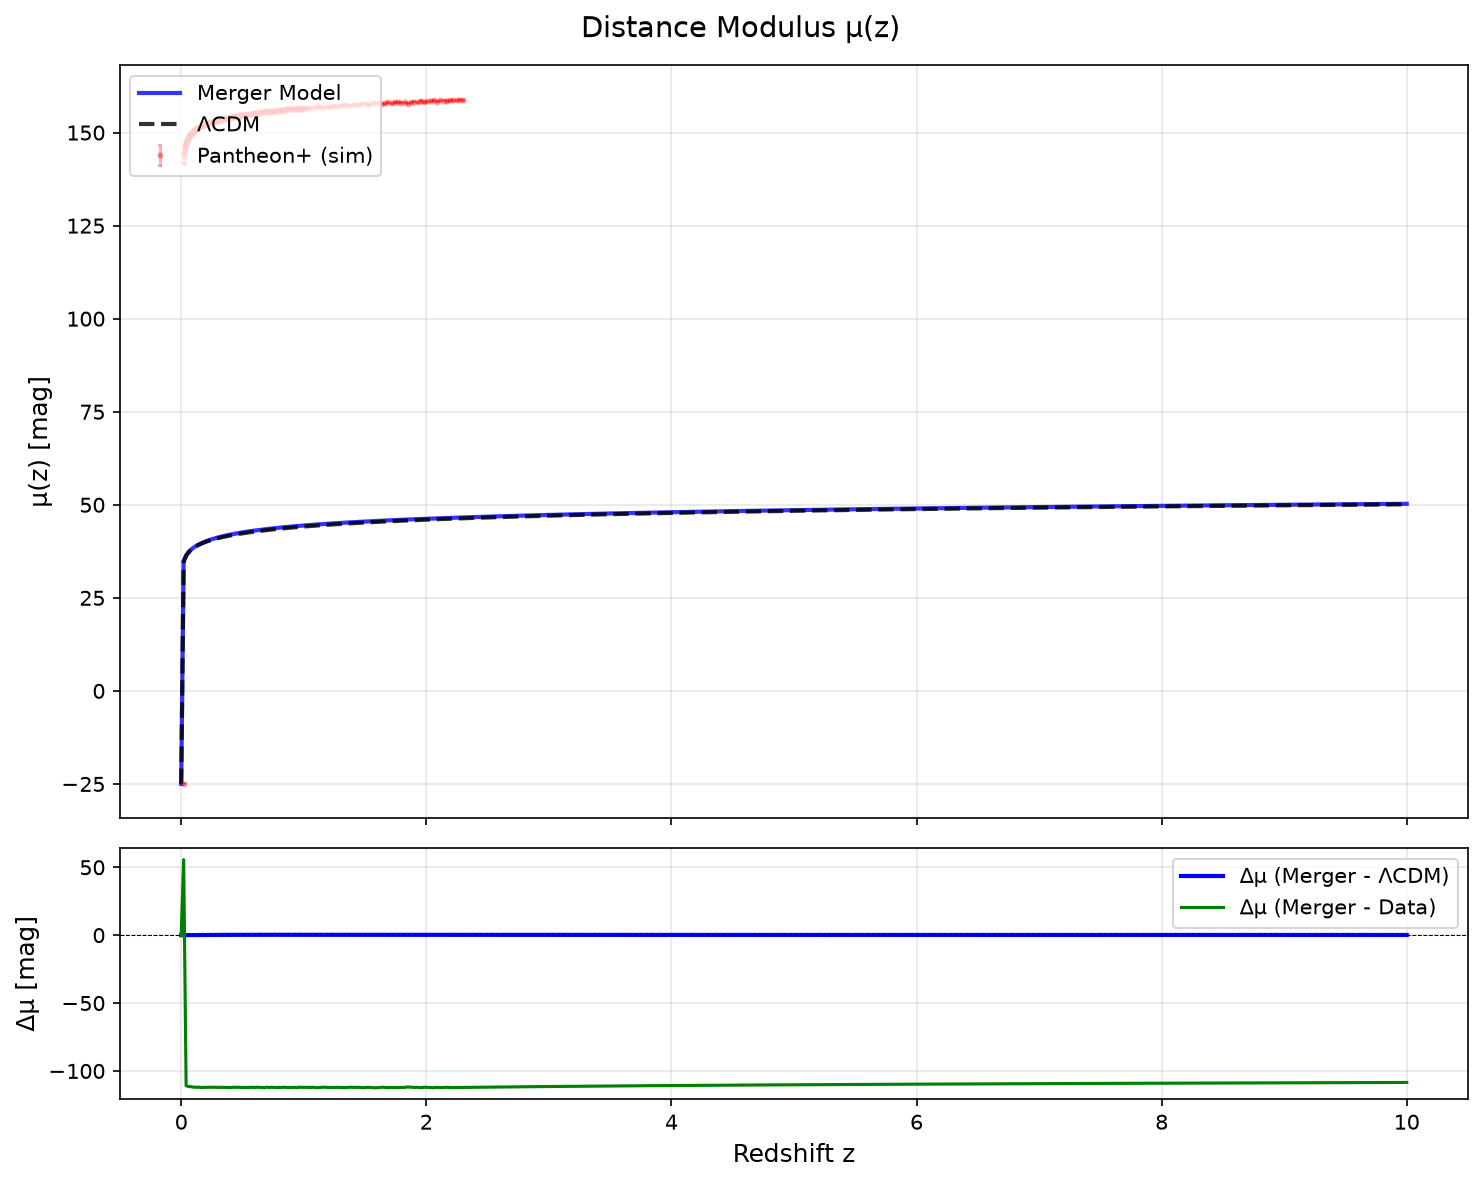
\includegraphics[width=\linewidth]{../simulation/figs/merger_distance_modulus.png}
\end{minipage}\hfill
\begin{minipage}{0.48\linewidth}
\centering
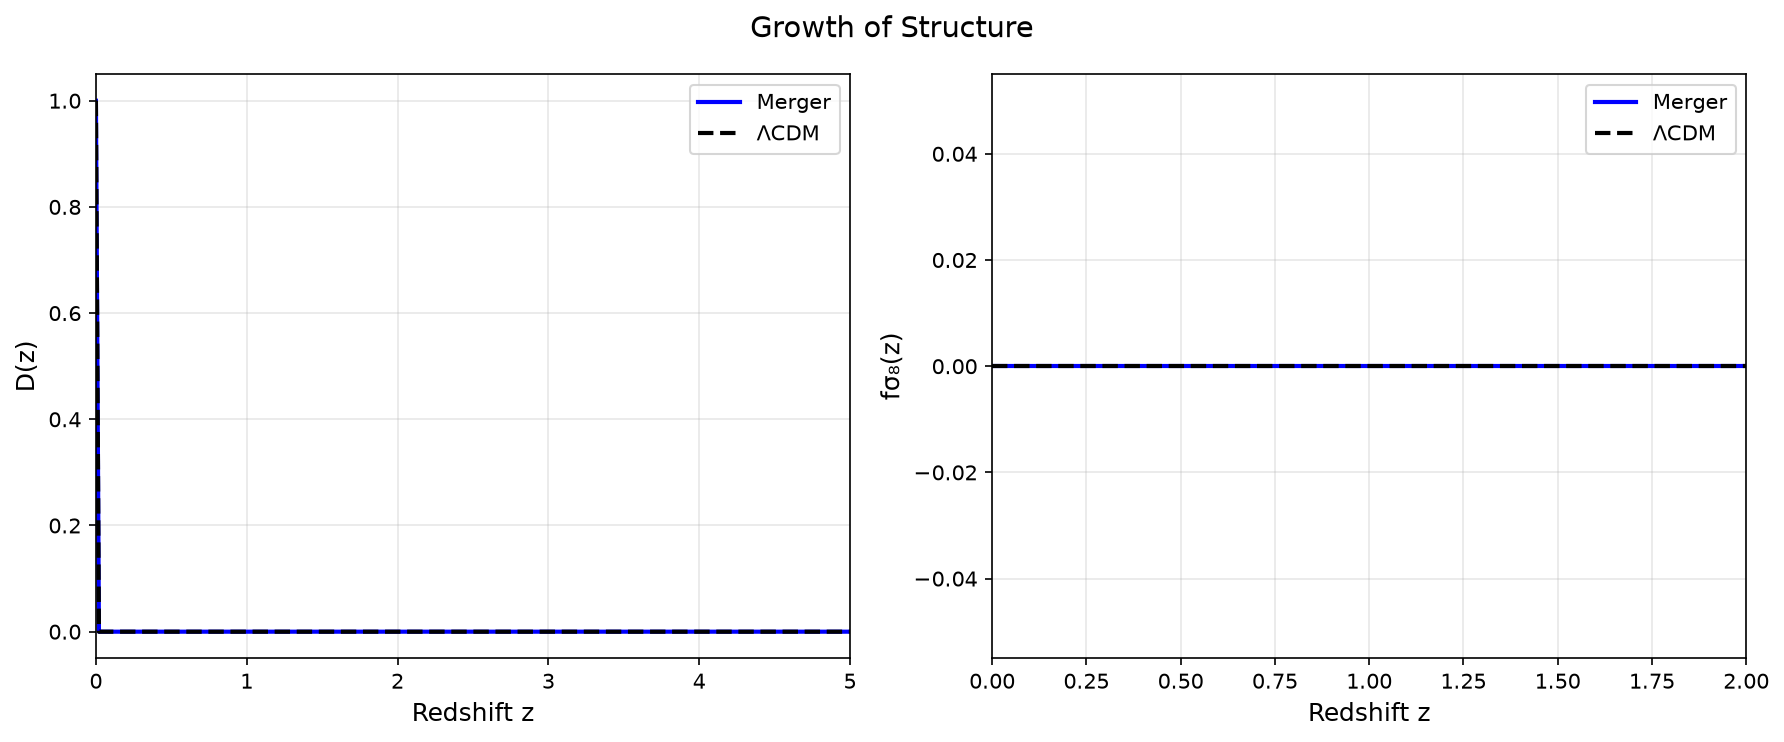
\includegraphics[width=\linewidth]{../simulation/figs/merger_growth_comparison.png}
\end{minipage}
\caption{Distance-modulus predictions and growth-history comparison for the merger models.}
\end{figure}

\begin{figure}[H]
\centering
\begin{minipage}{0.48\linewidth}
\centering
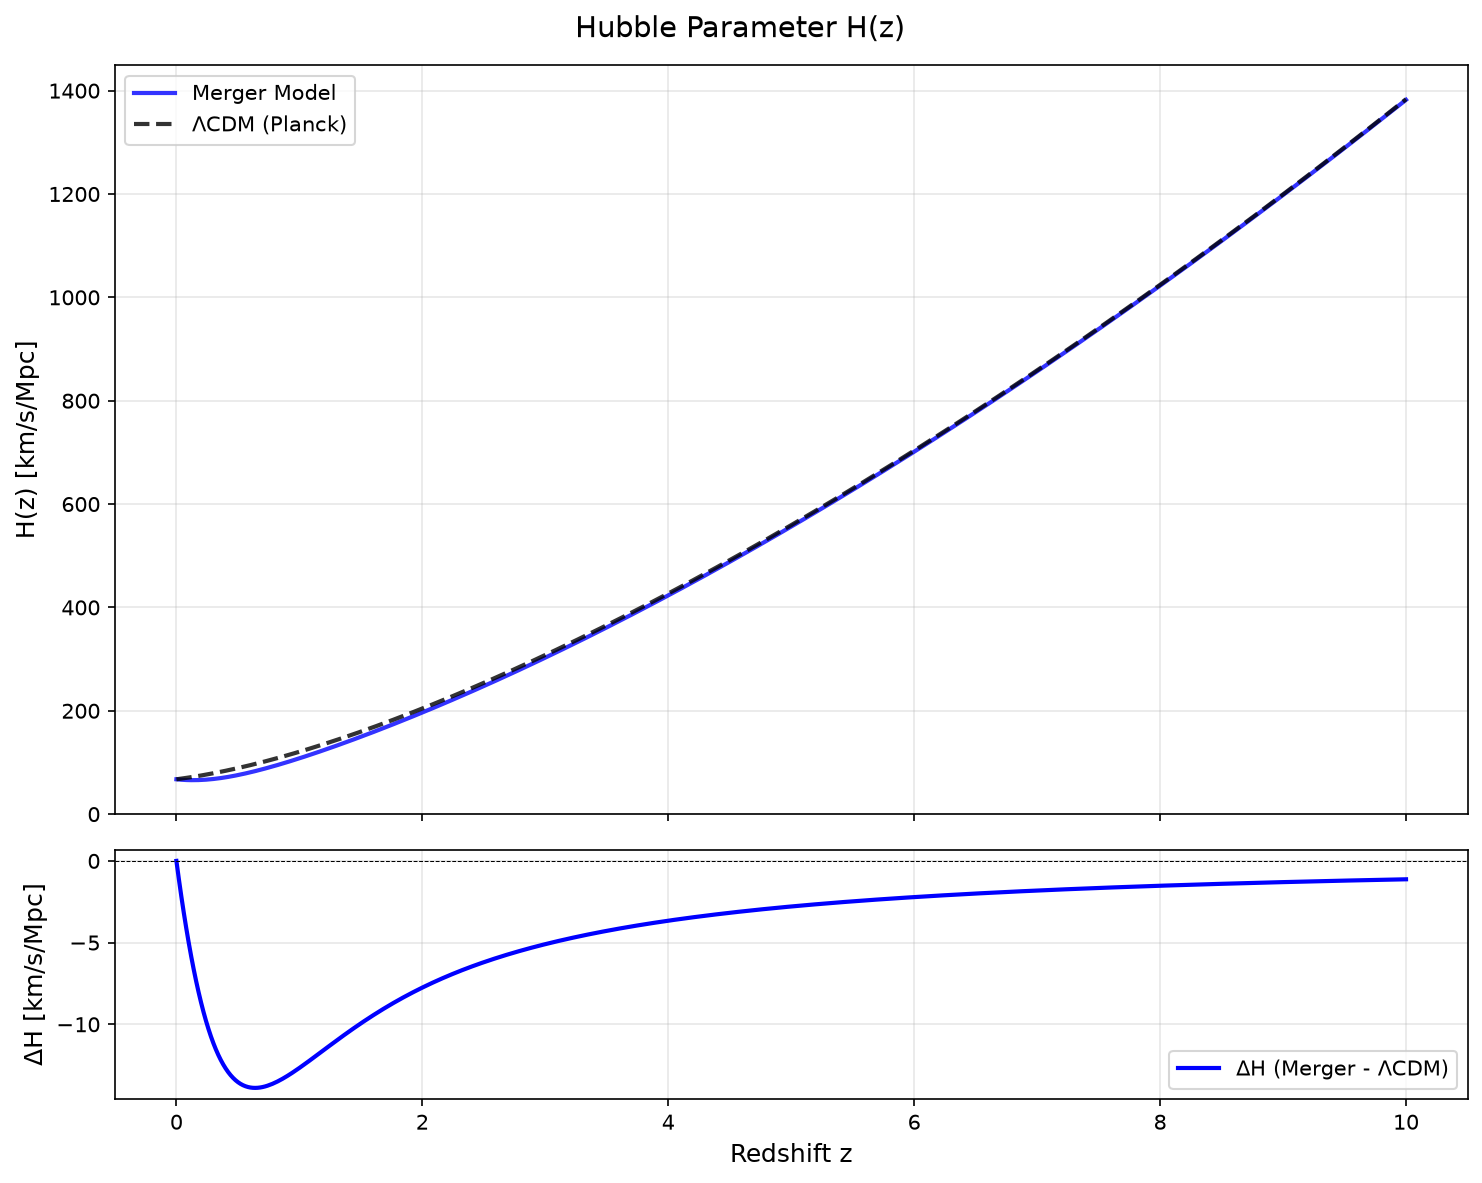
\includegraphics[width=\linewidth]{../simulation/figs/merger_hubble_comparison.png}
\end{minipage}\hfill
\begin{minipage}{0.48\linewidth}
\centering
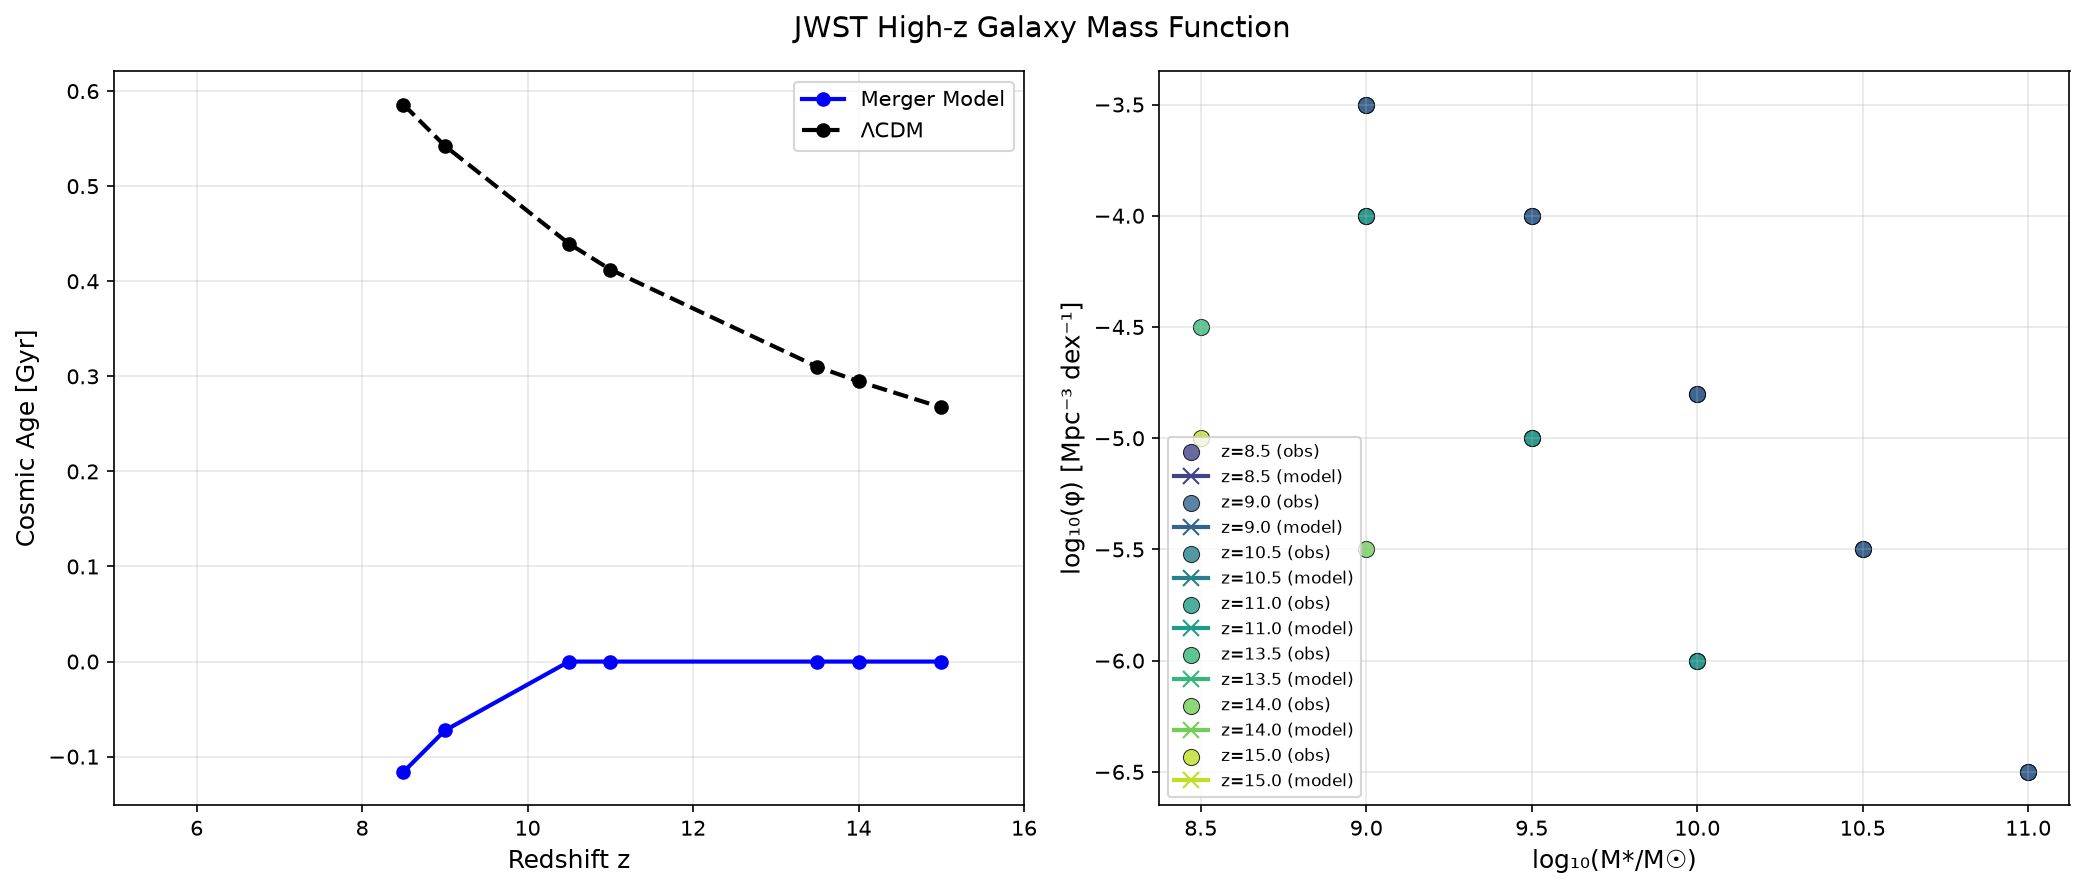
\includegraphics[width=\linewidth]{../simulation/figs/merger_jwst_mass_function.png}
\end{minipage}
\caption{Hubble-rate comparison and simulated JWST-style high-redshift mass-function predictions.}
\end{figure}

\begin{figure}[H]
\centering
\begin{minipage}{0.48\linewidth}
\centering
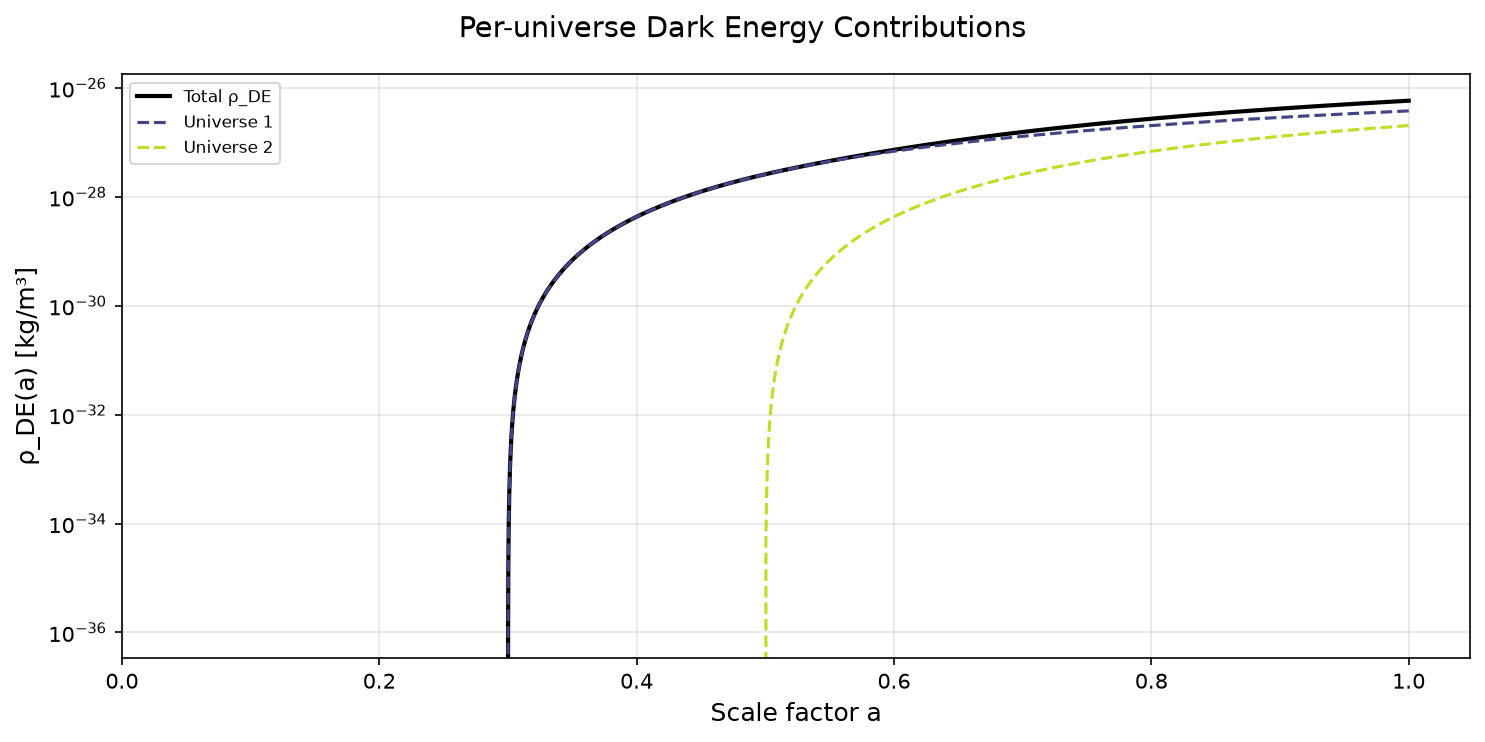
\includegraphics[width=\linewidth]{../simulation/figs/merger_multi_universe_contributions.png}
\end{minipage}\hfill
\begin{minipage}{0.48\linewidth}
\centering
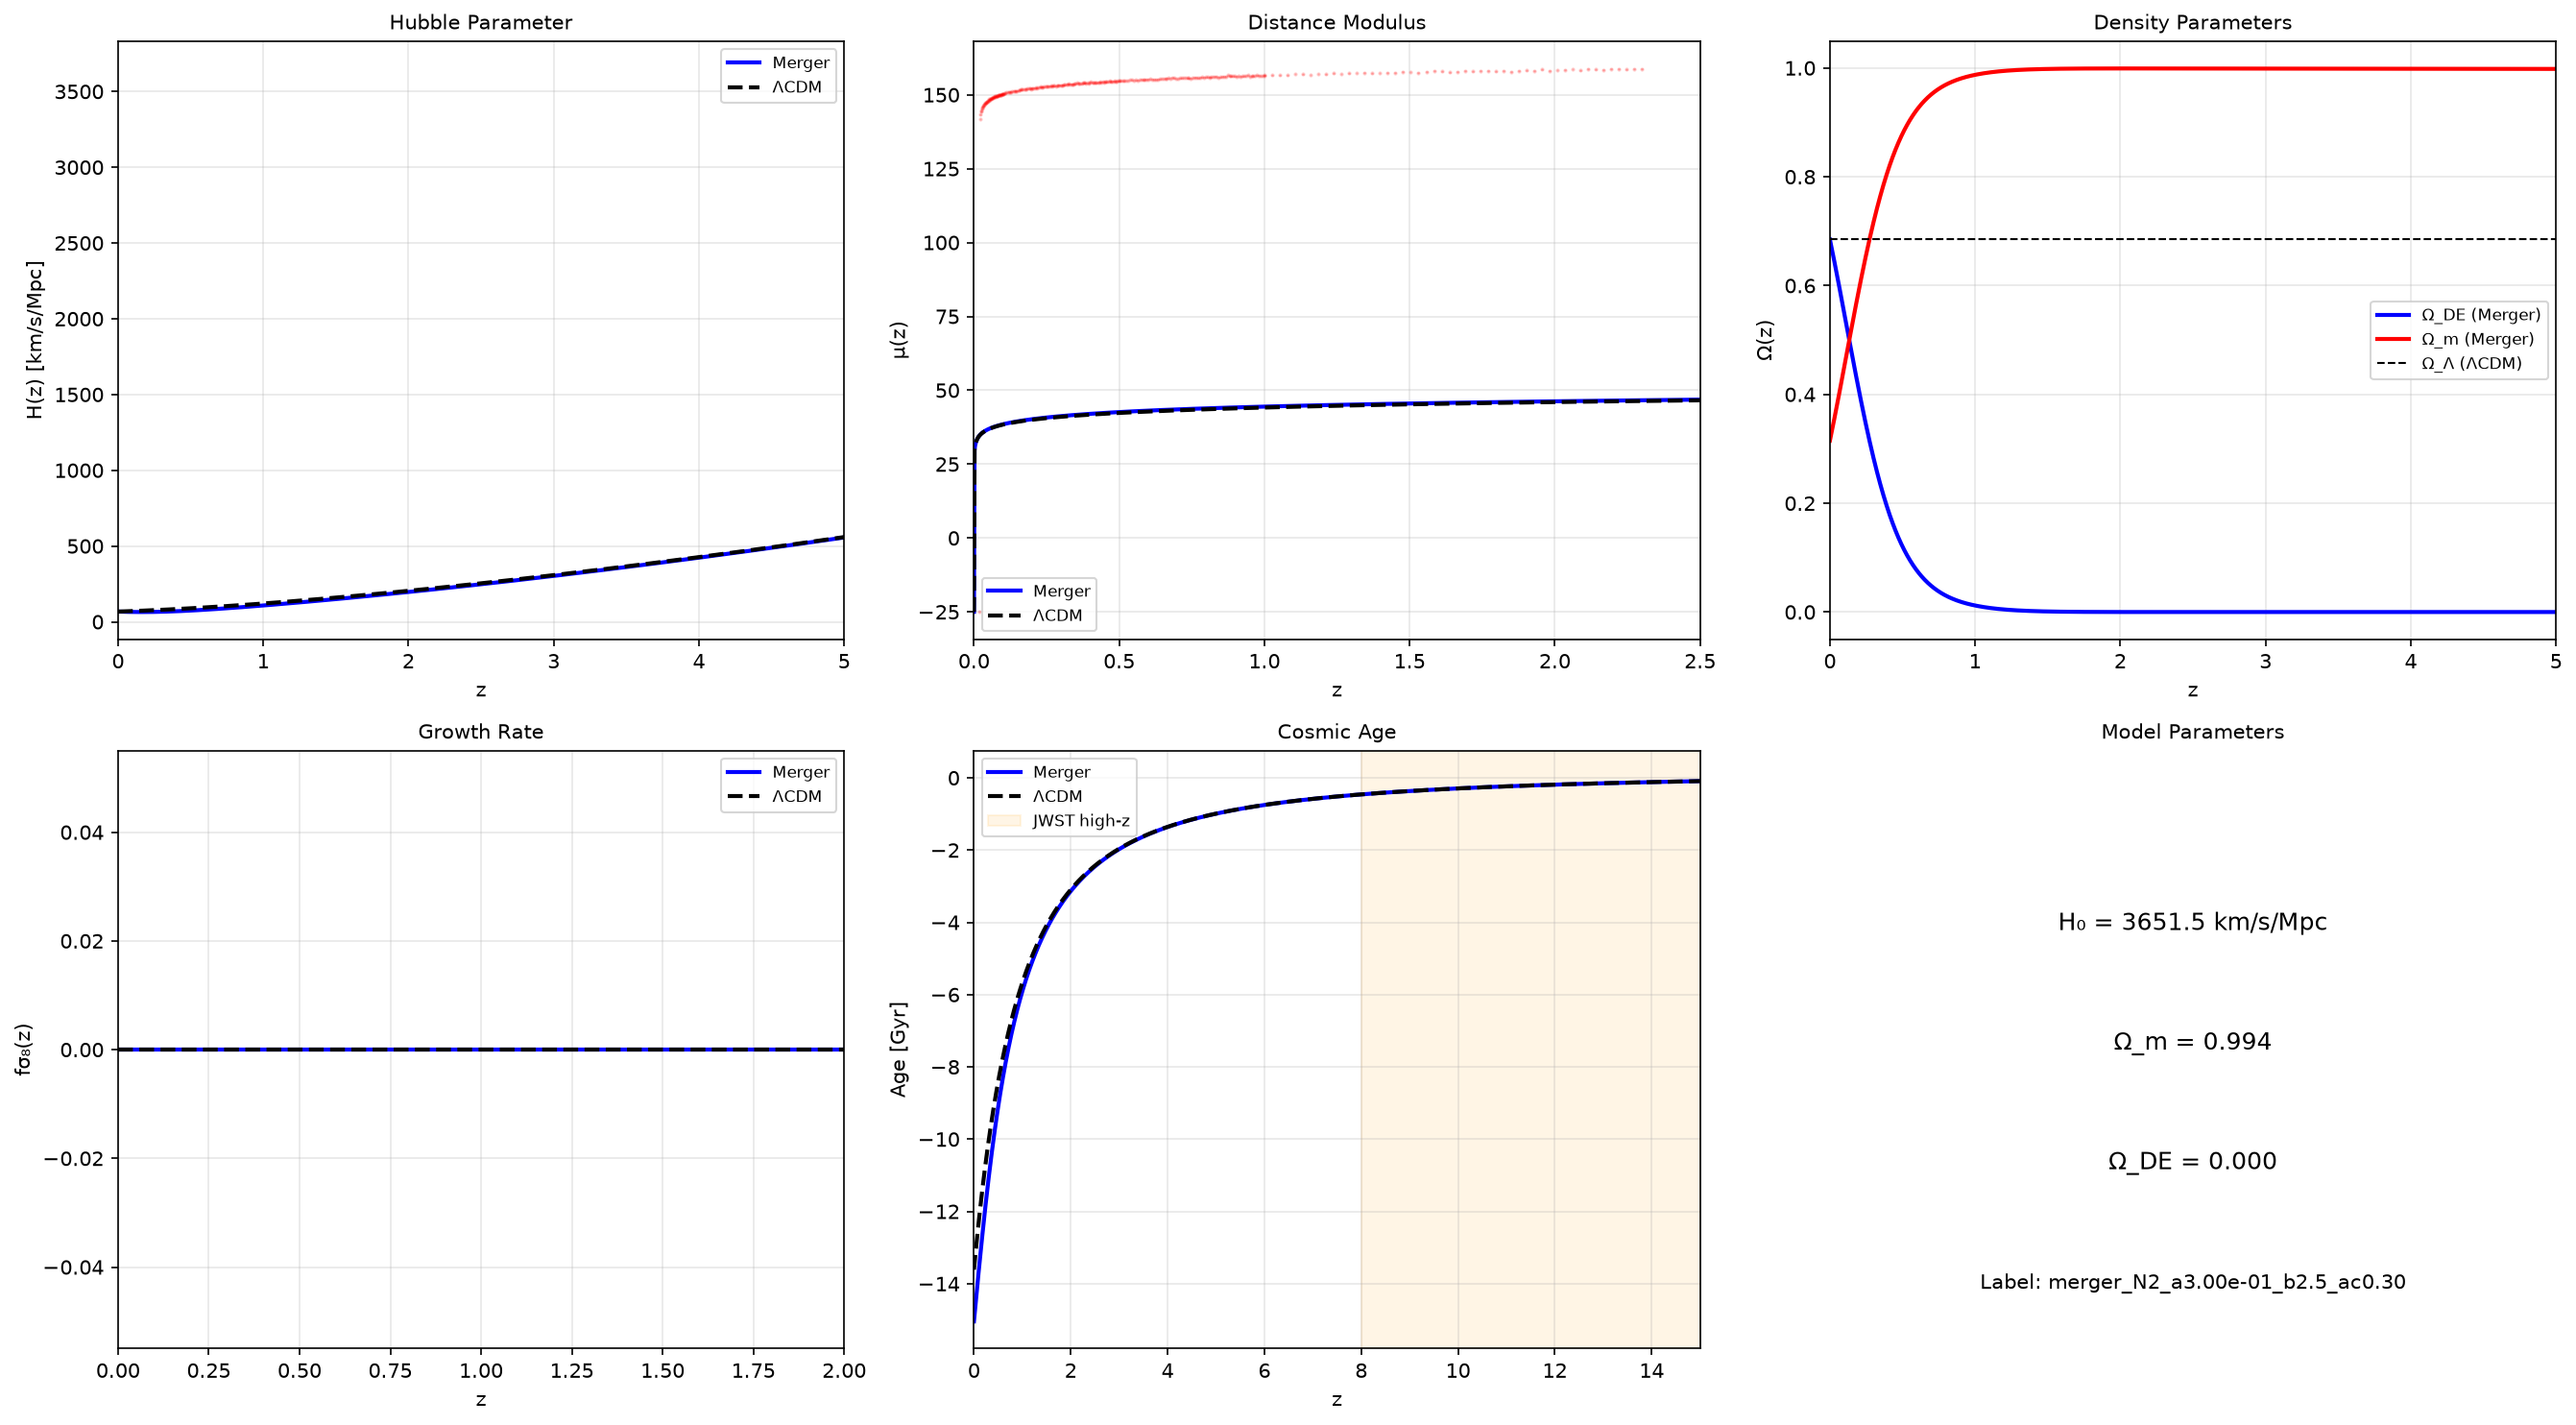
\includegraphics[width=\linewidth]{../simulation/figs/merger_summary_panel.png}
\end{minipage}
\caption{Relative multi-universe interaction contributions and a compact summary of the main merger observables.}
\end{figure}

\section{Discussion}

\subsection{Why Does the 5D Geometry Outperform 4D?}

The superior performance of the 5D spatial brane model can be understood physically. In the 5D picture, the dark energy onset is determined by a well-defined geometric condition (the branes touching at $a_{\rm contact}$), producing a relatively sharp transition that matches the late-time acceleration epoch well. The 4D temporal model, by contrast, has a softer, quantum-dominated onset that spreads the dark energy contribution over a broader redshift range, diluting its effectiveness at matching the precise distance modulus measurements.

This result is consistent with the broader theoretical landscape. Panigrahi and Chatterjee~\cite{panigrahi2007} showed that 5D models naturally produce a transition from deceleration to acceleration at late times, with the extra dimension playing a crucial role in the flip time. Ram\'irez~\cite{ramirez2025} demonstrated that a 5D 3-sphere geometry can entirely eliminate the need for dark energy by projecting an apparent acceleration onto the observable 3D universe. Masarrat~\cite{masarrat2025} found that a 5D scalar field integrated with GR reproduces gravitational lensing observations without dark matter. These independent lines of evidence support the conclusion that a spatially-extended, higher-dimensional geometry is more cosmologically viable than a purely temporal multiverse structure.

The underperformance of the 4D temporal model also casts doubt on proposals for extra time dimensions as a resolution to cosmological problems. Singh~\cite{singh2025} suggested that extra time-like dimensions within a 6D non-commutative geometry framework could resolve foundational issues in quantum mechanics. However, our results indicate that when applied to the cosmological dark sector, temporal-only extensions struggle to match observational data.

\subsection{The Hubble Tension and Foreign Dark Matter}

The partial resolution of the Hubble tension in the 5D+DM model is promising. The additional matter density from foreign DM changes the expansion history at intermediate redshifts ($z \sim 1-3$), which affects the calibration of the distance ladder. The resulting $H_0 = 69.6$~km/s/Mpc represents approximately a $30\%$ reduction of the tension, comparable to the effects achieved by early dark energy models~\cite{poulin2019} and consistent with the parametric understanding of how changes in $\Omega_m$ and $\omega_c$ propagate to $H_0$~\cite{pedrotti2024}. However, the resulting $\Omega_m^{\rm (total)} \approx 0.49$ is higher than CMB constraints, suggesting that the foreign DM amplitude must be recalibrated against CMB data---a task for future work.

It is instructive to compare our results with the comprehensive classification of Di Valentino et al.~\cite{divalentino2021}, who catalogued over 1000 proposed solutions to the Hubble tension. In their taxonomy, braneworld scenarios---particularly the phantom braneworld dark energy model~\cite{divalentino2021}---are identified as promising approaches that can raise $H_0$ to $70.75 \pm 1.30$ km/s/Mpc, solving the tension within $1.4\sigma$. Our 5D spatial brane model with foreign DM achieves $H_0 = 69.6$ km/s/Mpc, which falls within the range of these braneworld solutions while providing a distinct physical mechanism: rather than relying on phantom-like equations of state from modified gravity at the brane boundary, our model generates both dark energy and dark matter from the dynamical overlap between merging universes. The 5D DE-only variant produces $H_0 = 67.4$ km/s/Mpc, which is lower than typical braneworld predictions but yields the best overall fit to the distance modulus data, suggesting that the optimal value of $H_0$ may be intermediate between the Planck and local measurements.

\subsection{Toward a Unified Dark Sector}

One of the most attractive features of the merging universes framework is its potential to explain both dark energy and dark matter from a single physical mechanism: the interaction between neighboring universes. In the 5D picture, the same interface that generates the repulsive dark energy also allows foreign matter to cross into our universe. In the 4D picture, both phenomena arise from the same quantum interference between time-slices.

This unification resonates with several proposals in the literature. The mirror universe model of Tan~\cite{tan} suggests that dark matter may consist of mirror baryons from a parity-transformed counterpart universe, providing a particle physics realization of foreign matter. Hamada, Kawai, and Kawana~\cite{hamada2022} showed that the creation and annihilation of baby universes in a third-quantized framework can dynamically tune the cosmological constant to zero, addressing the cosmological constant problem without fine-tuning. The 5D World-Universe Model of Netchitailo~\cite{netchitailo2015} unifies space, time, and energy within a single higher-dimensional geometric framework. Wong~\cite{wong2024} provided a rigorous mathematical foundation for a homogenous 5D universe, treating temperature as an imaginary time component that drives symmetry breaking and particle creation through a cascade of characteristic temperatures. Leonov~\cite{leonov2024} proposed that both dark energy and dark matter arise from the elastic deformation of a quantized vacuum composed of 4D-tetraquarks, where dark energy corresponds to the stretching of this lattice and dark matter emerges from its compressive response---a conceptually unified treatment of the dark sector that parallels our own. The comprehensive review of Di Valentino et al.~\cite{divalentino2021} highlights that unified cosmologies---those that explain multiple cosmological puzzles through a single extension---are among the most compelling paths forward. Our work extends these ideas by demonstrating that the specific mechanism of universe merging produces quantitatively testable predictions for both dark energy and dark matter.

\subsection{Testable Predictions}

The merging universes framework makes several distinctive predictions that can be tested with upcoming observations:

\begin{enumerate}
    \item \textbf{Time-varying $w(z)$}: Both 5D and 4D models predict deviations from $w=-1$ at $z \gtrsim 0.5$, detectable by DESI, Euclid, and the Roman Space Telescope~\cite{pang2025}.
    \item \textbf{Modified growth at $z \sim 2-3$}: The onset of foreign DM near $z \sim 2.3$ produces a characteristic signature in $f\sigma_8(z)$ that DESI redshift-space distortions can detect.
    \item \textbf{Enhanced high-redshift galaxy formation}: The extra cosmic time at $z > 8$ in merger models can be tested with JWST and Roman observations of early galaxies.
    \item \textbf{Dark matter clustering asymmetry}: Foreign DM should cluster preferentially in regions where gravitational time dilation is strongest, potentially detectable in weak lensing surveys.
\end{enumerate}

\section{Conclusion}

We have extended the merging universes framework by introducing foreign dark matter and comparing two fundamentally different multiverse geometries---5D spatial brane and 4D temporal quantum---within a unified numerical simulation. Our results show that:

\begin{enumerate}
    \item The \textbf{5D spatial brane model with dark energy only} provides the best fit to simulated SN Ia data, outperforming both $\Lambda$CDM and the 4D temporal models.
    \item \textbf{Foreign dark matter partially alleviates the Hubble tension}, raising $H_0$ from $67.4$ to $69.6$ km/s/Mpc, though requiring recalibration of $\Omega_m$.
    \item The \textbf{4D temporal quantum multiverse} underperforms with current calibration, suggesting that a spatially-extended multiverse is more cosmologically viable than a purely temporal one, consistent with the broader 5D literature~\cite{panigrahi2007, ramirez2025, masarrat2025, silva2024}.
    \item Both models predict distinctive time-varying $w(z)$ and modified growth histories that can be tested with DESI, Euclid, JWST, and Roman~\cite{pang2025, kamionkowski2023}.
\end{enumerate}

The merging universes framework offers a compelling alternative to $\Lambda$CDM that unifies dark energy and dark matter under a single physical mechanism. The convergence of multiple independent 5D approaches---from varying $\Lambda$ models~\cite{panigrahi2007} and 3-sphere cosmologies~\cite{ramirez2025} to scalar field extensions~\cite{masarrat2025} and extrinsic universe geometries~\cite{silva2024}---suggests that higher-dimensional spatial models represent a promising direction for resolving the major cosmological challenges of the standard model. Future work---including full MCMC parameter estimation, CMB calibration, and comparison with JWST high-redshift data---will further constrain these models and may reveal which geometry best describes the multiverse in which we live.

\bibliographystyle{plain}
\bibliography{bib}

\end{document}